\section{细分曲面}\label{sec:细分曲面}
\begin{remark}
    本节含有高级内容,第一次阅读时可以跳过。
\end{remark}

本章我们要定义的最后一个形状表示
实现了\keyindex{细分曲面}{subdivision surface}{surface曲面},
该表示尤其适合描述复杂光滑形状。
特定网格的细分曲面定义为将网格面反复细分为更小面
然后用旧顶点位置的加权组合求新顶点位置。

对于适当选择的细分规则,当细分步数趋于无穷时,
该过程会收敛到给出一个光滑的\keyindex{极限曲面}{limit surface}{surface曲面}。
实践中,只需少量级别的细分通常就足以得到极限曲面的良好近似。
\reffig{3.24}展示了一个细分的简单例子,
其中四面体被细分了零次、一次、两次和六次。
\begin{figure}[htbp]
    \centering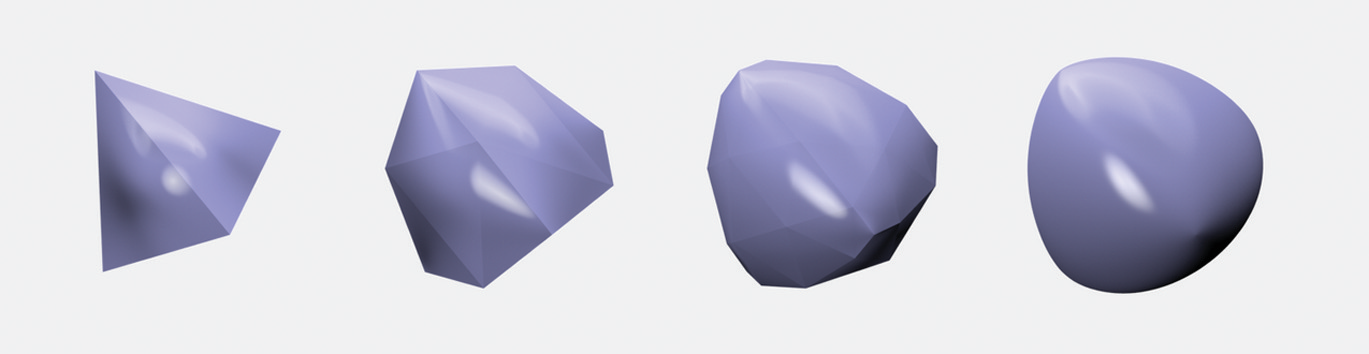
\includegraphics[width=\linewidth]{chap03/tetsubdiv.png}
    \caption{四面体的细分。从左到右使用了零步、一步、两步和六步细分
        (在零级时,顶点只是移动到极限曲面上)。
        随着细分得越来越多,网格逼近极限曲面,即原始网格描述的光滑曲面。
        随着执行更多级别的细分,注意高光如何变得更加准确、轮廓边缘如何变得更加平滑。}
    \label{fig:3.24}
\end{figure}

\reffig{3.25}展示了对Killeroo\sidenote{译者注:猜测此名字与一澳大利亚漫画中的袋鼠角色名有关。}模型应用细分的效果;
上面是原始控制网格,下面是控制网格表示的细分曲面。
\begin{figure}[htbp]
    \centering
    \subfloat[控制网格]{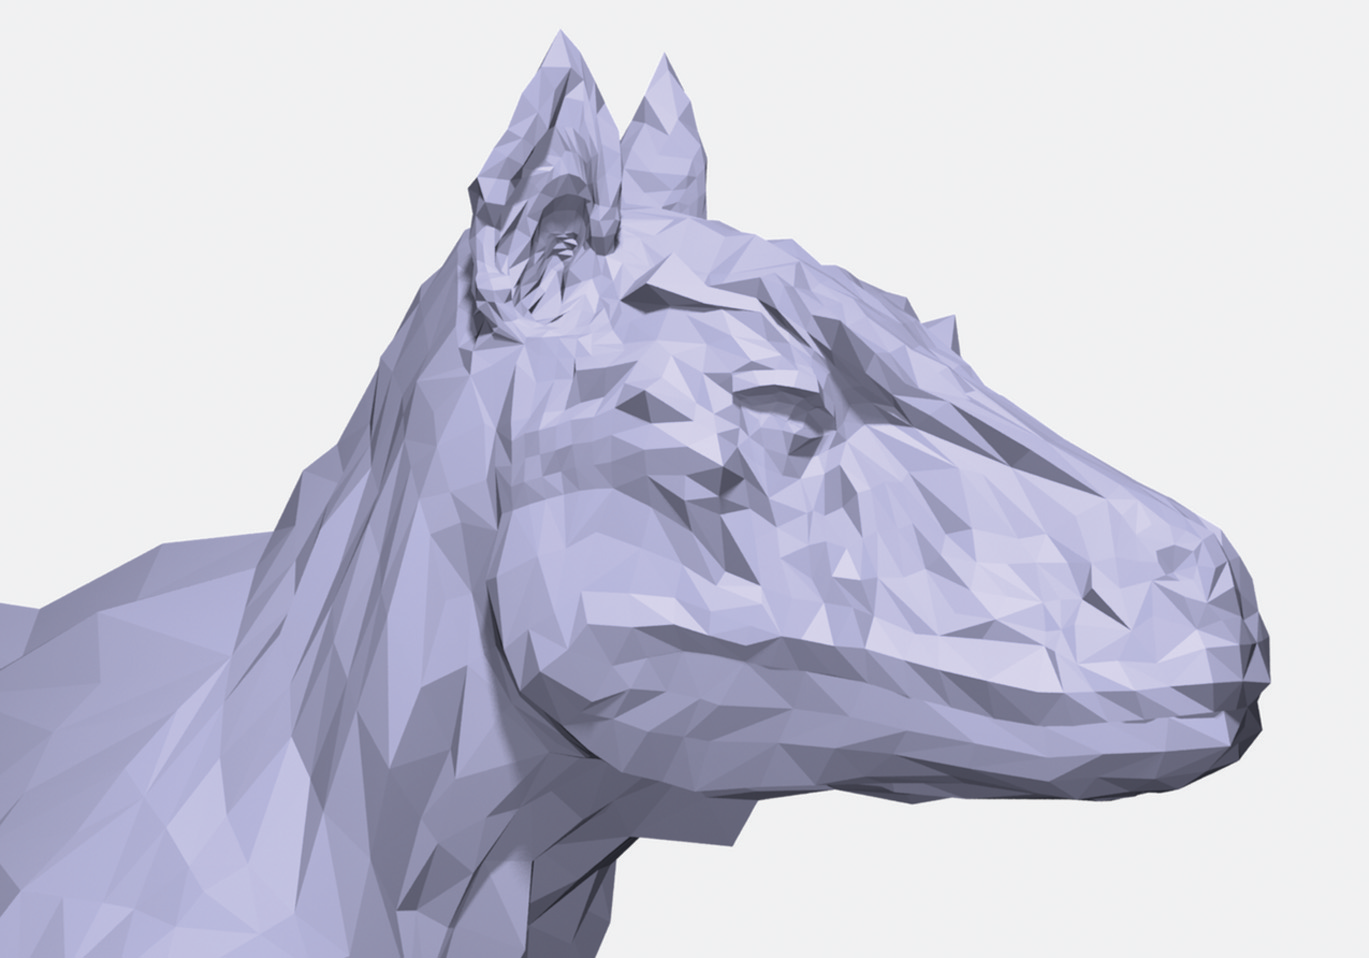
\includegraphics[width=\linewidth]{chap03/killeroo-control.png}\label{fig:3.25.1}}\\
    \subfloat[细分网格]{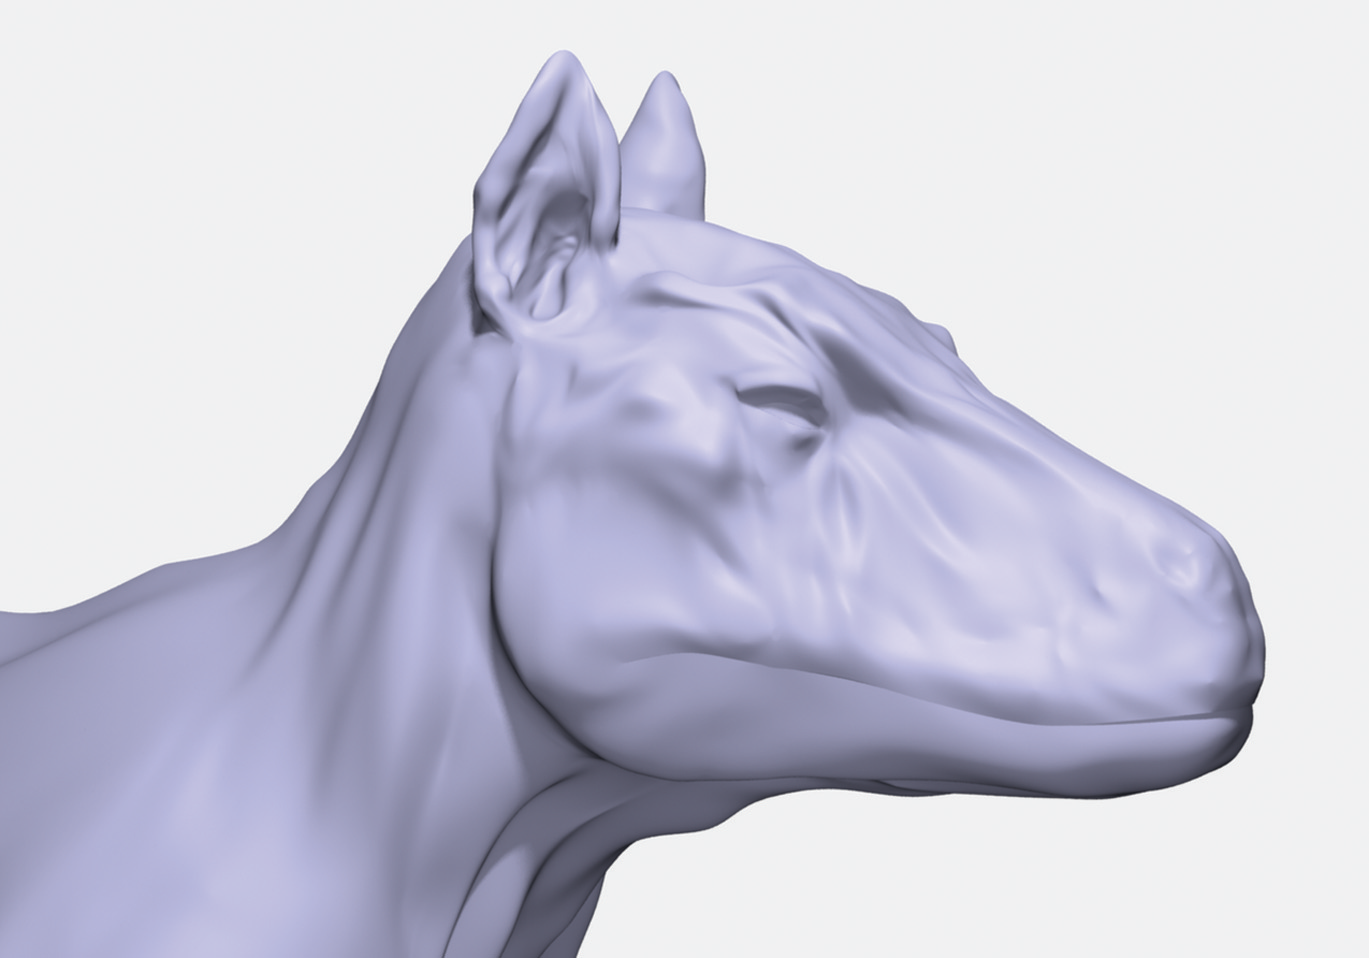
\includegraphics[width=\linewidth]{chap03/killeroo-subdivided.png}\label{fig:3.25.2}}
    \caption{对Killeroo模型应用细分。(1)控制网格描述了(2)结果细分曲面。
        细分非常适合建模这样的形状,因为它能通过细化控制网格轻松添加局部细节,
        对最终曲面没有拓扑结构限制。(模型由headus/Rezard提供。)}
    \label{fig:3.25}
\end{figure}


因为在曲面的多边形和基于样条的表示方面有一些重要优势,
细分曲面近年来得到广泛运用,尽管它在20世纪70年代就被发明了。
细分的优势包括:
\begin{itemize}
    \item 细分曲面是平滑的,而多边形网格与之相反,无论建模得多细致,靠近观察会有小面。
    \item 建模系统中现有的多数基本结构可以重定向到细分。
          建模多边形网格的经典技术工具箱可以应用到建模细分控制网格上。
    \item 细分曲面非常适合描述有复杂拓扑结构的物体,
          因为它们以任意(\keyindex{流形}{manifold}{})拓扑结构的控制网格为起点。
          参数化曲面模型一般不能很好地处理复杂拓扑结构。
    \item 细分方法常常是基于样条的曲面表示的推广,
          所以样条曲面常常可以由通用细分曲面渲染器运行。
    \item 通过简单地对控制网格的适当部分添加面,它能轻松对细分曲面局部区域添加细节。
          用样条表示则要困难得多。
\end{itemize}
\begin{figure}[htbp]
    \centering%LaTeX with PSTricks extensions
%%Creator: Inkscape 1.0.1 (3bc2e813f5, 2020-09-07)
%%Please note this file requires PSTricks extensions
\psset{xunit=.5pt,yunit=.5pt,runit=.5pt}
\begin{pspicture}(487.94000244,169.97000122)
{
\newrgbcolor{curcolor}{0.7019608 0.7019608 0.7019608}
\pscustom[linestyle=none,fillstyle=solid,fillcolor=curcolor]
{
\newpath
\moveto(96.28,168.97000122)
\lineto(143.98,86.34000122)
\lineto(191.69,3.72000122)
\lineto(96.28,3.72000122)
\lineto(0.87,3.72000122)
\lineto(48.57,86.34000122)
\closepath
}
}
{
\newrgbcolor{curcolor}{0 0 0}
\pscustom[linewidth=1,linecolor=curcolor]
{
\newpath
\moveto(96.28,168.97000122)
\lineto(143.98,86.34000122)
\lineto(191.69,3.72000122)
\lineto(96.28,3.72000122)
\lineto(0.87,3.72000122)
\lineto(48.57,86.34000122)
\closepath
}
}
{
\newrgbcolor{curcolor}{0.7019608 0.7019608 0.7019608}
\pscustom[linestyle=none,fillstyle=solid,fillcolor=curcolor]
{
\newpath
\moveto(96.28,4.73000122)
\lineto(72.9,45.22000122)
\lineto(49.52,85.71000122)
\lineto(96.28,85.71000122)
\lineto(143.03,85.71000122)
\lineto(119.65,45.22000122)
\closepath
}
}
{
\newrgbcolor{curcolor}{0 0 0}
\pscustom[linewidth=0.5,linecolor=curcolor]
{
\newpath
\moveto(96.28,4.73000122)
\lineto(72.9,45.22000122)
\lineto(49.52,85.71000122)
\lineto(96.28,85.71000122)
\lineto(143.03,85.71000122)
\lineto(119.65,45.22000122)
\closepath
}
}
{
\newrgbcolor{curcolor}{0.7019608 0.7019608 0.7019608}
\pscustom[linestyle=none,fillstyle=solid,fillcolor=curcolor]
{
\newpath
\moveto(391.67,168.97000122)
\lineto(439.37,86.34000122)
\lineto(487.08,3.72000122)
\lineto(391.67,3.72000122)
\lineto(296.26,3.72000122)
\lineto(343.96,86.34000122)
\closepath
}
}
{
\newrgbcolor{curcolor}{0 0 0}
\pscustom[linewidth=1,linecolor=curcolor]
{
\newpath
\moveto(391.67,168.97000122)
\lineto(439.37,86.34000122)
\lineto(487.08,3.72000122)
\lineto(391.67,3.72000122)
\lineto(296.26,3.72000122)
\lineto(343.96,86.34000122)
\closepath
}
}
{
\newrgbcolor{curcolor}{0.7019608 0.7019608 0.7019608}
\pscustom[linestyle=none,fillstyle=solid,fillcolor=curcolor]
{
\newpath
\moveto(391.67,4.73000122)
\lineto(368.29,45.22000122)
\lineto(344.92,85.71000122)
\lineto(391.67,85.71000122)
\lineto(438.42,85.71000122)
\lineto(415.04,45.22000122)
\closepath
}
}
{
\newrgbcolor{curcolor}{0 0 0}
\pscustom[linewidth=0.5,linecolor=curcolor]
{
\newpath
\moveto(391.67,4.73000122)
\lineto(368.29,45.22000122)
\lineto(344.92,85.71000122)
\lineto(391.67,85.71000122)
\lineto(438.42,85.71000122)
\lineto(415.04,45.22000122)
\closepath
}
}
{
\newrgbcolor{curcolor}{0.7019608 0.7019608 0.7019608}
\pscustom[linestyle=none,fillstyle=solid,fillcolor=curcolor]
{
\newpath
\moveto(391.89,86.41000122)
\lineto(380.43,106.25000122)
\lineto(368.98,126.09000122)
\lineto(391.89,126.09000122)
\lineto(414.8,126.09000122)
\lineto(403.34,106.25000122)
\closepath
}
}
{
\newrgbcolor{curcolor}{0 0 0}
\pscustom[linewidth=0.5,linecolor=curcolor,linestyle=dashed,dash=2]
{
\newpath
\moveto(391.89,86.41000122)
\lineto(380.43,106.25000122)
\lineto(368.98,126.09000122)
\lineto(391.89,126.09000122)
\lineto(414.8,126.09000122)
\lineto(403.34,106.25000122)
\closepath
}
}
{
\newrgbcolor{curcolor}{0.7019608 0.7019608 0.7019608}
\pscustom[linestyle=none,fillstyle=solid,fillcolor=curcolor]
{
\newpath
\moveto(344.09,4.78000122)
\lineto(332.64,24.62000122)
\lineto(321.19,44.46000122)
\lineto(344.09,44.46000122)
\lineto(367,44.46000122)
\lineto(355.55,24.62000122)
\closepath
}
}
{
\newrgbcolor{curcolor}{0 0 0}
\pscustom[linewidth=0.5,linecolor=curcolor,linestyle=dashed,dash=2]
{
\newpath
\moveto(344.09,4.78000122)
\lineto(332.64,24.62000122)
\lineto(321.19,44.46000122)
\lineto(344.09,44.46000122)
\lineto(367,44.46000122)
\lineto(355.55,24.62000122)
\closepath
}
}
{
\newrgbcolor{curcolor}{0.7019608 0.7019608 0.7019608}
\pscustom[linestyle=none,fillstyle=solid,fillcolor=curcolor]
{
\newpath
\moveto(439.39,5.37000122)
\lineto(427.94,25.21000122)
\lineto(416.48,45.05000122)
\lineto(439.39,45.05000122)
\lineto(462.3,45.05000122)
\lineto(450.84,25.21000122)
\closepath
}
}
{
\newrgbcolor{curcolor}{0 0 0}
\pscustom[linewidth=0.5,linecolor=curcolor,linestyle=dashed,dash=2]
{
\newpath
\moveto(439.39,5.37000122)
\lineto(427.94,25.21000122)
\lineto(416.48,45.05000122)
\lineto(439.39,45.05000122)
\lineto(462.3,45.05000122)
\lineto(450.84,25.21000122)
\closepath
}
}
{
\newrgbcolor{curcolor}{0.7019608 0.7019608 0.7019608}
\pscustom[linestyle=none,fillstyle=solid,fillcolor=curcolor]
{
\newpath
\moveto(392.26,85.27000122)
\lineto(403.71,65.43000122)
\lineto(415.16,45.59000122)
\lineto(392.26,45.59000122)
\lineto(369.35,45.59000122)
\lineto(380.8,65.43000122)
\closepath
}
}
{
\newrgbcolor{curcolor}{0 0 0}
\pscustom[linewidth=0.5,linecolor=curcolor,linestyle=dashed,dash=2]
{
\newpath
\moveto(392.26,85.27000122)
\lineto(403.71,65.43000122)
\lineto(415.16,45.59000122)
\lineto(392.26,45.59000122)
\lineto(369.35,45.59000122)
\lineto(380.8,65.43000122)
\closepath
}
}
{
\newrgbcolor{curcolor}{0 0 0}
\pscustom[linestyle=none,fillstyle=solid,fillcolor=curcolor]
{
\newpath
\moveto(419.14999509,126.22999954)
\curveto(419.14999509,129.37511236)(415.34769602,130.94962069)(413.124035,128.72595966)
\curveto(410.90037397,126.50229864)(412.4748823,122.69999957)(415.61999512,122.69999957)
\curveto(418.76510794,122.69999957)(420.33961626,126.50229864)(418.11595524,128.72595966)
\curveto(415.89229421,130.94962069)(412.08999515,129.37511236)(412.08999515,126.22999954)
\curveto(412.08999515,123.08488672)(415.89229421,121.5103784)(418.11595524,123.73403942)
\curveto(420.33961626,125.95770045)(418.76510794,129.75999951)(415.61999512,129.75999951)
\curveto(412.4748823,129.75999951)(410.90037397,125.95770045)(413.124035,123.73403942)
\curveto(415.34769602,121.5103784)(419.14999509,123.08488672)(419.14999509,126.22999954)
\closepath
}
}
{
\newrgbcolor{curcolor}{0 0 0}
\pscustom[linewidth=1,linecolor=curcolor]
{
\newpath
\moveto(419.14999509,126.22999954)
\curveto(419.14999509,129.37511236)(415.34769602,130.94962069)(413.124035,128.72595966)
\curveto(410.90037397,126.50229864)(412.4748823,122.69999957)(415.61999512,122.69999957)
\curveto(418.76510794,122.69999957)(420.33961626,126.50229864)(418.11595524,128.72595966)
\curveto(415.89229421,130.94962069)(412.08999515,129.37511236)(412.08999515,126.22999954)
\curveto(412.08999515,123.08488672)(415.89229421,121.5103784)(418.11595524,123.73403942)
\curveto(420.33961626,125.95770045)(418.76510794,129.75999951)(415.61999512,129.75999951)
\curveto(412.4748823,129.75999951)(410.90037397,125.95770045)(413.124035,123.73403942)
\curveto(415.34769602,121.5103784)(419.14999509,123.08488672)(419.14999509,126.22999954)
\closepath
}
}
{
\newrgbcolor{curcolor}{0 0 0}
\pscustom[linestyle=none,fillstyle=solid,fillcolor=curcolor]
{
\newpath
\moveto(395.51001096,85.79000092)
\curveto(395.51001096,88.93511374)(391.70771189,90.50962206)(389.48405087,88.28596104)
\curveto(387.26038984,86.06230001)(388.83489817,82.26000094)(391.98001099,82.26000094)
\curveto(395.12512381,82.26000094)(396.69963213,86.06230001)(394.47597111,88.28596104)
\curveto(392.25231008,90.50962206)(388.45001101,88.93511374)(388.45001101,85.79000092)
\curveto(388.45001101,82.6448881)(392.25231008,81.07037977)(394.47597111,83.2940408)
\curveto(396.69963213,85.51770182)(395.12512381,89.32000089)(391.98001099,89.32000089)
\curveto(388.83489817,89.32000089)(387.26038984,85.51770182)(389.48405087,83.2940408)
\curveto(391.70771189,81.07037977)(395.51001096,82.6448881)(395.51001096,85.79000092)
\closepath
}
}
{
\newrgbcolor{curcolor}{0 0 0}
\pscustom[linewidth=1,linecolor=curcolor]
{
\newpath
\moveto(395.51001096,85.79000092)
\curveto(395.51001096,88.93511374)(391.70771189,90.50962206)(389.48405087,88.28596104)
\curveto(387.26038984,86.06230001)(388.83489817,82.26000094)(391.98001099,82.26000094)
\curveto(395.12512381,82.26000094)(396.69963213,86.06230001)(394.47597111,88.28596104)
\curveto(392.25231008,90.50962206)(388.45001101,88.93511374)(388.45001101,85.79000092)
\curveto(388.45001101,82.6448881)(392.25231008,81.07037977)(394.47597111,83.2940408)
\curveto(396.69963213,85.51770182)(395.12512381,89.32000089)(391.98001099,89.32000089)
\curveto(388.83489817,89.32000089)(387.26038984,85.51770182)(389.48405087,83.2940408)
\curveto(391.70771189,81.07037977)(395.51001096,82.6448881)(395.51001096,85.79000092)
\closepath
}
}
{
\newrgbcolor{curcolor}{0 0 0}
\pscustom[linestyle=none,fillstyle=solid,fillcolor=curcolor]
{
\newpath
\moveto(370.98999143,127.18000031)
\curveto(370.98999143,130.32511313)(367.18769236,131.89962145)(364.96403134,129.67596042)
\curveto(362.74037031,127.4522994)(364.31487864,123.65000033)(367.45999146,123.65000033)
\curveto(370.60510428,123.65000033)(372.1796126,127.4522994)(369.95595157,129.67596042)
\curveto(367.73229055,131.89962145)(363.92999148,130.32511313)(363.92999148,127.18000031)
\curveto(363.92999148,124.03488749)(367.73229055,122.46037916)(369.95595157,124.68404019)
\curveto(372.1796126,126.90770121)(370.60510428,130.71000028)(367.45999146,130.71000028)
\curveto(364.31487864,130.71000028)(362.74037031,126.90770121)(364.96403134,124.68404019)
\curveto(367.18769236,122.46037916)(370.98999143,124.03488749)(370.98999143,127.18000031)
\closepath
}
}
{
\newrgbcolor{curcolor}{0 0 0}
\pscustom[linewidth=1,linecolor=curcolor]
{
\newpath
\moveto(370.98999143,127.18000031)
\curveto(370.98999143,130.32511313)(367.18769236,131.89962145)(364.96403134,129.67596042)
\curveto(362.74037031,127.4522994)(364.31487864,123.65000033)(367.45999146,123.65000033)
\curveto(370.60510428,123.65000033)(372.1796126,127.4522994)(369.95595157,129.67596042)
\curveto(367.73229055,131.89962145)(363.92999148,130.32511313)(363.92999148,127.18000031)
\curveto(363.92999148,124.03488749)(367.73229055,122.46037916)(369.95595157,124.68404019)
\curveto(372.1796126,126.90770121)(370.60510428,130.71000028)(367.45999146,130.71000028)
\curveto(364.31487864,130.71000028)(362.74037031,126.90770121)(364.96403134,124.68404019)
\curveto(367.18769236,122.46037916)(370.98999143,124.03488749)(370.98999143,127.18000031)
\closepath
}
}
{
\newrgbcolor{curcolor}{0 0 0}
\pscustom[linestyle=none,fillstyle=solid,fillcolor=curcolor]
{
\newpath
\moveto(418.45999265,46.02999878)
\curveto(418.45999265,49.1751116)(414.65769358,50.74961993)(412.43403256,48.5259589)
\curveto(410.21037153,46.30229787)(411.78487986,42.49999881)(414.92999268,42.49999881)
\curveto(418.0751055,42.49999881)(419.64961382,46.30229787)(417.4259528,48.5259589)
\curveto(415.20229177,50.74961993)(411.3999927,49.1751116)(411.3999927,46.02999878)
\curveto(411.3999927,42.88488596)(415.20229177,41.31037763)(417.4259528,43.53403866)
\curveto(419.64961382,45.75769969)(418.0751055,49.55999875)(414.92999268,49.55999875)
\curveto(411.78487986,49.55999875)(410.21037153,45.75769969)(412.43403256,43.53403866)
\curveto(414.65769358,41.31037763)(418.45999265,42.88488596)(418.45999265,46.02999878)
\closepath
}
}
{
\newrgbcolor{curcolor}{0 0 0}
\pscustom[linewidth=1,linecolor=curcolor]
{
\newpath
\moveto(418.45999265,46.02999878)
\curveto(418.45999265,49.1751116)(414.65769358,50.74961993)(412.43403256,48.5259589)
\curveto(410.21037153,46.30229787)(411.78487986,42.49999881)(414.92999268,42.49999881)
\curveto(418.0751055,42.49999881)(419.64961382,46.30229787)(417.4259528,48.5259589)
\curveto(415.20229177,50.74961993)(411.3999927,49.1751116)(411.3999927,46.02999878)
\curveto(411.3999927,42.88488596)(415.20229177,41.31037763)(417.4259528,43.53403866)
\curveto(419.64961382,45.75769969)(418.0751055,49.55999875)(414.92999268,49.55999875)
\curveto(411.78487986,49.55999875)(410.21037153,45.75769969)(412.43403256,43.53403866)
\curveto(414.65769358,41.31037763)(418.45999265,42.88488596)(418.45999265,46.02999878)
\closepath
}
}
{
\newrgbcolor{curcolor}{0 0 0}
\pscustom[linestyle=none,fillstyle=solid,fillcolor=curcolor]
{
\newpath
\moveto(371.64999509,45.45000458)
\curveto(371.64999509,48.5951174)(367.84769602,50.16962572)(365.624035,47.9459647)
\curveto(363.40037397,45.72230367)(364.9748823,41.92000461)(368.11999512,41.92000461)
\curveto(371.26510794,41.92000461)(372.83961626,45.72230367)(370.61595524,47.9459647)
\curveto(368.39229421,50.16962572)(364.58999515,48.5951174)(364.58999515,45.45000458)
\curveto(364.58999515,42.30489176)(368.39229421,40.73038343)(370.61595524,42.95404446)
\curveto(372.83961626,45.17770548)(371.26510794,48.98000455)(368.11999512,48.98000455)
\curveto(364.9748823,48.98000455)(363.40037397,45.17770548)(365.624035,42.95404446)
\curveto(367.84769602,40.73038343)(371.64999509,42.30489176)(371.64999509,45.45000458)
\closepath
}
}
{
\newrgbcolor{curcolor}{0 0 0}
\pscustom[linewidth=1,linecolor=curcolor]
{
\newpath
\moveto(371.64999509,45.45000458)
\curveto(371.64999509,48.5951174)(367.84769602,50.16962572)(365.624035,47.9459647)
\curveto(363.40037397,45.72230367)(364.9748823,41.92000461)(368.11999512,41.92000461)
\curveto(371.26510794,41.92000461)(372.83961626,45.72230367)(370.61595524,47.9459647)
\curveto(368.39229421,50.16962572)(364.58999515,48.5951174)(364.58999515,45.45000458)
\curveto(364.58999515,42.30489176)(368.39229421,40.73038343)(370.61595524,42.95404446)
\curveto(372.83961626,45.17770548)(371.26510794,48.98000455)(368.11999512,48.98000455)
\curveto(364.9748823,48.98000455)(363.40037397,45.17770548)(365.624035,42.95404446)
\curveto(367.84769602,40.73038343)(371.64999509,42.30489176)(371.64999509,45.45000458)
\closepath
}
}
{
\newrgbcolor{curcolor}{0 0 0}
\pscustom[linestyle=none,fillstyle=solid,fillcolor=curcolor]
{
\newpath
\moveto(466.45999265,45.13999939)
\curveto(466.45999265,48.28511221)(462.65769358,49.85962054)(460.43403256,47.63595951)
\curveto(458.21037153,45.41229848)(459.78487986,41.60999942)(462.92999268,41.60999942)
\curveto(466.0751055,41.60999942)(467.64961382,45.41229848)(465.4259528,47.63595951)
\curveto(463.20229177,49.85962054)(459.3999927,48.28511221)(459.3999927,45.13999939)
\curveto(459.3999927,41.99488657)(463.20229177,40.42037824)(465.4259528,42.64403927)
\curveto(467.64961382,44.8677003)(466.0751055,48.66999936)(462.92999268,48.66999936)
\curveto(459.78487986,48.66999936)(458.21037153,44.8677003)(460.43403256,42.64403927)
\curveto(462.65769358,40.42037824)(466.45999265,41.99488657)(466.45999265,45.13999939)
\closepath
}
}
{
\newrgbcolor{curcolor}{0 0 0}
\pscustom[linewidth=1,linecolor=curcolor]
{
\newpath
\moveto(466.45999265,45.13999939)
\curveto(466.45999265,48.28511221)(462.65769358,49.85962054)(460.43403256,47.63595951)
\curveto(458.21037153,45.41229848)(459.78487986,41.60999942)(462.92999268,41.60999942)
\curveto(466.0751055,41.60999942)(467.64961382,45.41229848)(465.4259528,47.63595951)
\curveto(463.20229177,49.85962054)(459.3999927,48.28511221)(459.3999927,45.13999939)
\curveto(459.3999927,41.99488657)(463.20229177,40.42037824)(465.4259528,42.64403927)
\curveto(467.64961382,44.8677003)(466.0751055,48.66999936)(462.92999268,48.66999936)
\curveto(459.78487986,48.66999936)(458.21037153,44.8677003)(460.43403256,42.64403927)
\curveto(462.65769358,40.42037824)(466.45999265,41.99488657)(466.45999265,45.13999939)
\closepath
}
}
{
\newrgbcolor{curcolor}{0 0 0}
\pscustom[linestyle=none,fillstyle=solid,fillcolor=curcolor]
{
\newpath
\moveto(323.7000134,45.41999817)
\curveto(323.7000134,48.56511099)(319.89771433,50.13961932)(317.67405331,47.91595829)
\curveto(315.45039228,45.69229726)(317.02490061,41.8899982)(320.17001343,41.8899982)
\curveto(323.31512625,41.8899982)(324.88963457,45.69229726)(322.66597355,47.91595829)
\curveto(320.44231252,50.13961932)(316.64001346,48.56511099)(316.64001346,45.41999817)
\curveto(316.64001346,42.27488535)(320.44231252,40.70037702)(322.66597355,42.92403805)
\curveto(324.88963457,45.14769908)(323.31512625,48.94999814)(320.17001343,48.94999814)
\curveto(317.02490061,48.94999814)(315.45039228,45.14769908)(317.67405331,42.92403805)
\curveto(319.89771433,40.70037702)(323.7000134,42.27488535)(323.7000134,45.41999817)
\closepath
}
}
{
\newrgbcolor{curcolor}{0 0 0}
\pscustom[linewidth=1,linecolor=curcolor]
{
\newpath
\moveto(323.7000134,45.41999817)
\curveto(323.7000134,48.56511099)(319.89771433,50.13961932)(317.67405331,47.91595829)
\curveto(315.45039228,45.69229726)(317.02490061,41.8899982)(320.17001343,41.8899982)
\curveto(323.31512625,41.8899982)(324.88963457,45.69229726)(322.66597355,47.91595829)
\curveto(320.44231252,50.13961932)(316.64001346,48.56511099)(316.64001346,45.41999817)
\curveto(316.64001346,42.27488535)(320.44231252,40.70037702)(322.66597355,42.92403805)
\curveto(324.88963457,45.14769908)(323.31512625,48.94999814)(320.17001343,48.94999814)
\curveto(317.02490061,48.94999814)(315.45039228,45.14769908)(317.67405331,42.92403805)
\curveto(319.89771433,40.70037702)(323.7000134,42.27488535)(323.7000134,45.41999817)
\closepath
}
}
{
\newrgbcolor{curcolor}{0 0 0}
\pscustom[linestyle=none,fillstyle=solid,fillcolor=curcolor]
{
\newpath
\moveto(347.83999753,4.04000854)
\curveto(347.83999753,7.18512136)(344.03769847,8.75962969)(341.81403744,6.53596866)
\curveto(339.59037641,4.31230764)(341.16488474,0.51000857)(344.30999756,0.51000857)
\curveto(347.45511038,0.51000857)(349.0296187,4.31230764)(346.80595768,6.53596866)
\curveto(344.58229665,8.75962969)(340.77999759,7.18512136)(340.77999759,4.04000854)
\curveto(340.77999759,0.89489572)(344.58229665,-0.6796126)(346.80595768,1.54404843)
\curveto(349.0296187,3.76770945)(347.45511038,7.57000852)(344.30999756,7.57000852)
\curveto(341.16488474,7.57000852)(339.59037641,3.76770945)(341.81403744,1.54404843)
\curveto(344.03769847,-0.6796126)(347.83999753,0.89489572)(347.83999753,4.04000854)
\closepath
}
}
{
\newrgbcolor{curcolor}{0 0 0}
\pscustom[linewidth=1,linecolor=curcolor]
{
\newpath
\moveto(347.83999753,4.04000854)
\curveto(347.83999753,7.18512136)(344.03769847,8.75962969)(341.81403744,6.53596866)
\curveto(339.59037641,4.31230764)(341.16488474,0.51000857)(344.30999756,0.51000857)
\curveto(347.45511038,0.51000857)(349.0296187,4.31230764)(346.80595768,6.53596866)
\curveto(344.58229665,8.75962969)(340.77999759,7.18512136)(340.77999759,4.04000854)
\curveto(340.77999759,0.89489572)(344.58229665,-0.6796126)(346.80595768,1.54404843)
\curveto(349.0296187,3.76770945)(347.45511038,7.57000852)(344.30999756,7.57000852)
\curveto(341.16488474,7.57000852)(339.59037641,3.76770945)(341.81403744,1.54404843)
\curveto(344.03769847,-0.6796126)(347.83999753,0.89489572)(347.83999753,4.04000854)
\closepath
}
}
{
\newrgbcolor{curcolor}{0 0 0}
\pscustom[linestyle=none,fillstyle=solid,fillcolor=curcolor]
{
\newpath
\moveto(443.57000852,4.02999878)
\curveto(443.57000852,7.1751116)(439.76770945,8.74961993)(437.54404843,6.5259589)
\curveto(435.3203874,4.30229787)(436.89489572,0.49999881)(440.04000854,0.49999881)
\curveto(443.18512136,0.49999881)(444.75962969,4.30229787)(442.53596866,6.5259589)
\curveto(440.31230764,8.74961993)(436.51000857,7.1751116)(436.51000857,4.02999878)
\curveto(436.51000857,0.88488596)(440.31230764,-0.68962237)(442.53596866,1.53403866)
\curveto(444.75962969,3.75769969)(443.18512136,7.55999875)(440.04000854,7.55999875)
\curveto(436.89489572,7.55999875)(435.3203874,3.75769969)(437.54404843,1.53403866)
\curveto(439.76770945,-0.68962237)(443.57000852,0.88488596)(443.57000852,4.02999878)
\closepath
}
}
{
\newrgbcolor{curcolor}{0 0 0}
\pscustom[linewidth=1,linecolor=curcolor]
{
\newpath
\moveto(443.57000852,4.02999878)
\curveto(443.57000852,7.1751116)(439.76770945,8.74961993)(437.54404843,6.5259589)
\curveto(435.3203874,4.30229787)(436.89489572,0.49999881)(440.04000854,0.49999881)
\curveto(443.18512136,0.49999881)(444.75962969,4.30229787)(442.53596866,6.5259589)
\curveto(440.31230764,8.74961993)(436.51000857,7.1751116)(436.51000857,4.02999878)
\curveto(436.51000857,0.88488596)(440.31230764,-0.68962237)(442.53596866,1.53403866)
\curveto(444.75962969,3.75769969)(443.18512136,7.55999875)(440.04000854,7.55999875)
\curveto(436.89489572,7.55999875)(435.3203874,3.75769969)(437.54404843,1.53403866)
\curveto(439.76770945,-0.68962237)(443.57000852,0.88488596)(443.57000852,4.02999878)
\closepath
}
}
{
\newrgbcolor{curcolor}{0 0 0}
\pscustom[linewidth=1,linecolor=curcolor]
{
\newpath
\moveto(189.22000122,98.36000061)
\lineto(288.66000366,98.36000061)
}
}
{
\newrgbcolor{curcolor}{0 0 0}
\pscustom[linestyle=none,fillstyle=solid,fillcolor=curcolor]
{
\newpath
\moveto(283.75,92.85000122)
\lineto(288.01,98.36000122)
\lineto(283.75,103.86000122)
\lineto(296.76,98.36000122)
\closepath
}
}
{
\newrgbcolor{curcolor}{0.65098041 0.65098041 0.65098041}
\pscustom[linestyle=none,fillstyle=solid,fillcolor=curcolor]
{
\newpath
\moveto(285.31,94.06000122)
\lineto(295.45,98.36000122)
\lineto(288.64,98.36000122)
\closepath
}
}
{
\newrgbcolor{curcolor}{0.40000001 0.40000001 0.40000001}
\pscustom[linestyle=none,fillstyle=solid,fillcolor=curcolor]
{
\newpath
\moveto(285.31,102.66000122)
\lineto(295.45,98.36000122)
\lineto(288.64,98.36000122)
\closepath
}
}
\end{pspicture}

    \caption{Loop细分的基本细化过程。(左)细分之前的控制网格。
        (右)一步细分后的新网格。通过划分每条边并连接新顶点和新边,
        网格的每个三角形面都被细分为四个新面。}
    \label{fig:3.26}
\end{figure}

这里,我们将介绍\keyindex{Loop细分曲面}{Loop subdivision surface}{surface曲面}
\footnote{以所用的细分规则发明者Charles Loop的名字命名。}的一种实现。
Loop细分规则基于控制网格中的三角形面;
开始时具有超过三个顶点的面被三角剖分。
在每步细分中,所有面分为四个子面(\reffig{3.26})。
沿原始网格的所有边添加新顶点,
使用相邻顶点的加权平均计算位置。
而且,每个原始顶点的位置也用其位置和新邻居位置的加权平均更新。
这里的实现使用的权值基于Hoppe等\parencite*{10.1145/192161.192233}开发的
对Loop方法的改进。
我们这里不涵盖关于怎样推导出这些权值的讨论。
虽然需要精妙的数学推导证明它们确实满足了这一点,
但必须谨慎选择它们以保证极限曲面确实有特定期望的光滑性质。

细分曲面不是在pbrt中实现为\refvar{Shape}{},
而是由函数\refvar{LoopSubdivide}{()}推广,
它将细分规则应用到一系列顶点和顶点索引表示的网格上
并返回表示最终细分网格的\refvar{Triangle}{}向量。
\begin{lstlisting}
`\initcode{LoopSubdiv Function Definitions}{=}\initnext{LoopSubdivFunctionDefinitions}`
std::vector<std::shared_ptr<`\refvar{Shape}{}`>> `\initvar{LoopSubdivide}{}`(
        const `\refvar{Transform}{}` *ObjectToWorld, const `\refvar{Transform}{}` *WorldToObject,
        bool reverseOrientation, int nLevels, int nIndices,
        const int *vertexIndices, int nVertices, const `\refvar{Point3f}{}` *p) {
    std::vector<`\refvar{SDVertex}{}` *> vertices;
    std::vector<`\refvar{SDFace}{}` *> faces;
    `\refcode{Allocate LoopSubdiv vertices and faces}{}`
    `\refcode{Set face to vertex pointers}{}`
    `\refcode{Set neighbor pointers in faces}{}`
    `\refcode{Finish vertex initialization}{}`
    `\refcode{Refine subdivision mesh into triangles}{}`
}
\end{lstlisting}

\subsection{网格表示}\label{sub:网格表示}
\refvar{LoopSubdivide}{()}的参数用和\refvar{TriangleMesh}{}构造函数中
一样的格式指定了三角网格(\refsec{三角形网格}):
每个面由三个整数顶点索引描述,
给出面的三个顶点在顶点数组{\ttfamily p}中的偏移量。
我们需要处理该数据以决定哪些面彼此相邻,
哪些面和哪些顶点相邻
\sidenote{译者注:文中“相邻”是一个宽泛的概念。
    面与面“相邻”指两个面有公共边;
    面与点“相邻”指该点是该面的顶点;
    面与边“相邻”指该边是该面的一条边。
    边与点“相邻”指该点是该边的端点……下文同。}等等,以实现细分算法。

我们将很快定义结构体\refvar{SDVertex}{}和\refvar{SDFace}{},
它们存有细分网格中顶点和面的数据。
\refvar{LoopSubdivide}{()}从为网格中的每个顶点分配
一个\refvar{SDVertex}{}实例以及为每个面分配\refvar{SDFace}{}开始。
现在,它们几乎都没有初始化。
\begin{lstlisting}
`\initcode{Allocate LoopSubdiv vertices and faces}{=}`
std::unique_ptr<`\refvar{SDVertex}{}`[]> verts(new `\refvar{SDVertex}{}`[nVertices]);
for (int i = 0; i < nVertices; ++i) {
    verts[i] = `\refvar{SDVertex}{}`(p[i]);
    vertices.push_back(&verts[i]);
}
int nFaces = nIndices / 3;
std::unique_ptr<`\refvar{SDFace}{}`[]> fs(new `\refvar{SDFace}{}`[nFaces]);
for (int i = 0; i < nFaces; ++i)
    faces.push_back(&fs[i]);
\end{lstlisting}

Loop细分方案像多数其他细分方案那样,
假设控制网格是\keyindex{流形}{manifold}{}——
共享任意给定边的面不超过两个。
这样的网格可能是闭合的或开放的:\keyindex{闭合网格}{closed mesh}{mesh网格}没有
边界且所有面的每条边都有邻接面。\keyindex{开放网格}{open mesh}{mesh网格}有
一些面没有全部三个邻居。
这里的实现同时支持闭合和开放网格。

在三角网格内部,大多数顶点和六个面相邻且
有六个相邻顶点通过边直接与其相连。
在开放网格的边界上,大多数顶点与三个面和四个顶点相邻。
与一个顶点直接相邻的顶点数称为该顶点的\keyindex{价}{valence}{}。
价不是六的内部顶点或价不是四的边界顶点
称为\keyindex{非凡顶点}{extraordinary vertex}{vertex顶点};
否则称为\keyindex{正则的}{regular}{}\footnote{这些术语常用于建模文献中,
    尽管“irregular”对“regular”或者“extraordinary”对“ordinary”更符合直觉。}。
Loop细分曲面在除非凡顶点外的任意处都是光滑的。

每个\refvar{SDVertex}{}存储其位置\refvar[SDVertex::p]{p}{}、
表示它是正则还是非凡顶点的布尔量以及
记录它是否位于网格边界上的布尔量。
它也存有指向任意与之相邻的面的指针;
该指针给出了寻找其所有相邻面的起点。
最后如果有的话,有一个指针为下一级的细分存储相应的\refvar{SDVertex}{}。
\begin{lstlisting}
`\initcode{LoopSubdiv Local Structures}{=}\initnext{LoopSubdivLocalStructures}`
struct `\initvar{SDVertex}{}` {
    `\refcode{SDVertex Constructor}{}`
    `\refcode{SDVertex Methods}{}`
    `\refvar{Point3f}{}` `\initvar[SDVertex::p]{p}{}`;
    `\refvar{SDFace}{}` *`\initvar{startFace}{}` = nullptr;
    `\refvar{SDVertex}{}` *`\initvar{child}{}` = nullptr;
    bool `\initvar{regular}{}` = false, `\initvar[SDVertex::boundary]{boundary}{}` = false;
};
\end{lstlisting}
\begin{lstlisting}
`\initcode{SDVertex Constructor}{=}`
`\refvar{SDVertex}{}`(const `\refvar{Point3f}{}` &p = `\refvar{Point3f}{}`(0, 0, 0)) : `\refvar[SDVertex::p]{p}{}`(p) { }
\end{lstlisting}

结构体\refvar{SDFace}{}存有最多关于网格的拓扑信息的地方。
因为所有面都是三角形,面总是存有指向其三个顶点的指针以及
指向其三条边相邻的面的指针。
如果面在开放网格边缘上则相应的相邻面指针为{\ttfamily nullptr}。

相邻面指针索引是,如果我们把从{\ttfamily\refvar[SDFace::v]{v}{}[i]}到{\ttfamily\refvar[SDFace::v]{v}{}[(i+1)\%3]}的边
标为第{\ttfamily i}边,则该边的相邻面存于{\ttfamily\refvar[SDFace::f]{f}{}[i]}(\reffig{3.27})。
\begin{figure}[htbp]
    \centering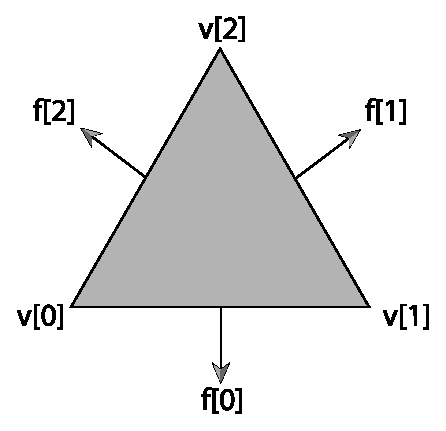
\includegraphics[width=0.35\linewidth]{chap03/Subdivvertfacepointers.eps}
    \caption{每个三角形面存有三个指向\protect\refvar{SDVertex}{}对象的
    指针{\ttfamily\protect\refvar[SDFace::v]{v}{}[i]}以及三个
    指向相邻面的指针{\ttfamily\protect\refvar[SDFace::f]{f}{}[i]}。
    相邻面索引使用的约定是第{\ttfamily i}边是
    从{\ttfamily\protect\refvar[SDFace::v]{v}{}[i]}到{\ttfamily\protect\refvar[SDFace::v]{v}{}[(i+1)\%3]}的边,
    且第{\ttfamily i}边的邻居在{\ttfamily\protect\refvar[SDFace::f]{f}{}[i]}中。}
    \label{fig:3.27}
\end{figure}

\begin{lstlisting}
`\refcode{LoopSubdiv Local Structures}{+=}\lastnext{LoopSubdivLocalStructures}`
struct `\initvar{SDFace}{}` {
    `\refcode{SDFace Constructor}{}`
    `\refcode{SDFace Methods}{}`
    `\refvar{SDVertex}{}` *`\initvar[SDFace::v]{v}{}`[3];
    `\refvar{SDFace}{}` *`\initvar[SDFace::f]{f}{}`[3];
    `\refvar{SDFace}{}` *`\initvar{children}{}`[4];
};
\end{lstlisting}

\refvar{SDFace}{}构造函数很简单——它简单地把这些不同的指针设置为{\ttfamily nullptr}——
所以这里不再展示。

为简化\refvar{SDFace}{}的数据结构导航,
我们提供宏使得决定特定索引前后的顶点和面索引更容易。
这些宏添加适合的偏移量并计算模三结果以负责循环。
\begin{lstlisting}
`\initcode{LoopSubdiv Macros}{=}`
#define `\initvar{NEXT}{}`(i) (((i) + 1) % 3)
#define `\initvar{PREV}{}`(i) (((i) + 2) % 3)
\end{lstlisting}

除了需要流形网格外,细分代码希望用户指定的控制网格
是\keyindex{相容次序}{consistently ordered}{}的——
网格中每条\keyindex{有向边}{directed edge}{edge边}只出现一次。
两个面的公共边须由每个面指定为不同方向。
考虑两个顶点$\bm v_0$和$\bm v_1$与连接它们的边。
我们希望拥有该边的三角形面指定其三个顶点时$\bm v_0$在$\bm v_1$之前,
另一个面指定顶点时$\bm v_1$在$\bm v_0$之前(\reffig{3.28})。
\keyindex{默比乌斯带}{Möbius strip}{}是无法相容次序的曲面例子,
但渲染中几乎不会遇到这样的曲面,所以实践中该限制没问题。
然而不能创建相容次序网格的程序给出的没构建好的网格数据可能会造成问题。
\begin{figure}[htbp]
    \centering%LaTeX with PSTricks extensions
%%Creator: Inkscape 1.0.1 (3bc2e813f5, 2020-09-07)
%%Please note this file requires PSTricks extensions
\psset{xunit=.4pt,yunit=.4pt,runit=.4pt}
\begin{pspicture}(341.97000122,255.44999695)
{
\newrgbcolor{curcolor}{0 0 0}
\pscustom[linewidth=1,linecolor=curcolor]
{
\newpath
\moveto(127.34,36.99999695)
\lineto(126.89,36.93999695)
\lineto(32.5,23.00999695)
\lineto(67.63,111.70999695)
}
}
{
\newrgbcolor{curcolor}{0 0 0}
\pscustom[linestyle=none,fillstyle=solid,fillcolor=curcolor]
{
\newpath
\moveto(121.67,41.72999695)
\lineto(126.69,36.90999695)
\lineto(123.28,30.83999695)
\lineto(135.35,38.18999695)
\closepath
}
}
{
\newrgbcolor{curcolor}{0.65098041 0.65098041 0.65098041}
\pscustom[linestyle=none,fillstyle=solid,fillcolor=curcolor]
{
\newpath
\moveto(123.39,40.76999695)
\lineto(134.06,37.98999695)
\lineto(127.32,36.99999695)
\closepath
}
}
{
\newrgbcolor{curcolor}{0.40000001 0.40000001 0.40000001}
\pscustom[linestyle=none,fillstyle=solid,fillcolor=curcolor]
{
\newpath
\moveto(124.65,32.25999695)
\lineto(134.06,37.98999695)
\lineto(127.32,36.99999695)
\closepath
}
}
{
\newrgbcolor{curcolor}{0 0 0}
\pscustom[linewidth=1,linecolor=curcolor]
{
\newpath
\moveto(67.63,111.70999695)
\lineto(102.77,200.41999695)
\lineto(162.02,125.63999695)
\lineto(162.59,124.91999695)
}
}
{
\newrgbcolor{curcolor}{0 0 0}
\pscustom[linestyle=none,fillstyle=solid,fillcolor=curcolor]
{
\newpath
\moveto(74.56,114.24999695)
\lineto(67.87,112.31999695)
\lineto(64.32,118.30999695)
\lineto(64.65,104.17999695)
\closepath
}
}
{
\newrgbcolor{curcolor}{0.65098041 0.65098041 0.65098041}
\pscustom[linestyle=none,fillstyle=solid,fillcolor=curcolor]
{
\newpath
\moveto(72.87,113.24999695)
\lineto(65.13,105.39999695)
\lineto(67.64,111.72999695)
\closepath
}
}
{
\newrgbcolor{curcolor}{0.40000001 0.40000001 0.40000001}
\pscustom[linestyle=none,fillstyle=solid,fillcolor=curcolor]
{
\newpath
\moveto(64.87,116.40999695)
\lineto(65.13,105.39999695)
\lineto(67.64,111.72999695)
\closepath
}
}
{
\newrgbcolor{curcolor}{0 0 0}
\pscustom[linewidth=1,linecolor=curcolor]
{
\newpath
\moveto(162.59,124.91999695)
\lineto(221.28,50.86999695)
\lineto(133.97,37.97999695)
}
}
{
\newrgbcolor{curcolor}{0 0 0}
\pscustom[linestyle=none,fillstyle=solid,fillcolor=curcolor]
{
\newpath
\moveto(161.33,117.65999695)
\lineto(163,124.40999695)
\lineto(169.95,124.48999695)
\lineto(157.56,131.27999695)
\closepath
}
}
{
\newrgbcolor{curcolor}{0.65098041 0.65098041 0.65098041}
\pscustom[linestyle=none,fillstyle=solid,fillcolor=curcolor]
{
\newpath
\moveto(161.3,119.62999695)
\lineto(158.37,130.24999695)
\lineto(162.6,124.90999695)
\closepath
}
}
{
\newrgbcolor{curcolor}{0.40000001 0.40000001 0.40000001}
\pscustom[linestyle=none,fillstyle=solid,fillcolor=curcolor]
{
\newpath
\moveto(168.04,124.96999695)
\lineto(158.37,130.24999695)
\lineto(162.6,124.90999695)
\closepath
}
}
{
\newrgbcolor{curcolor}{0 0 0}
\pscustom[linewidth=1,linecolor=curcolor]
{
\newpath
\moveto(270.07,144.47999695)
\lineto(269.9,144.05999695)
\lineto(234.64,55.40999695)
\lineto(175.5,130.26999695)
}
}
{
\newrgbcolor{curcolor}{0 0 0}
\pscustom[linestyle=none,fillstyle=solid,fillcolor=curcolor]
{
\newpath
\moveto(263.14,141.94999695)
\lineto(269.83,143.86999695)
\lineto(273.37,137.87999695)
\lineto(273.07,152.00999695)
\closepath
}
}
{
\newrgbcolor{curcolor}{0.65098041 0.65098041 0.65098041}
\pscustom[linestyle=none,fillstyle=solid,fillcolor=curcolor]
{
\newpath
\moveto(264.83,142.94999695)
\lineto(272.58,150.78999695)
\lineto(270.06,144.45999695)
\closepath
}
}
{
\newrgbcolor{curcolor}{0.40000001 0.40000001 0.40000001}
\pscustom[linestyle=none,fillstyle=solid,fillcolor=curcolor]
{
\newpath
\moveto(272.82,139.76999695)
\lineto(272.58,150.78999695)
\lineto(270.06,144.45999695)
\closepath
}
}
{
\newrgbcolor{curcolor}{0 0 0}
\pscustom[linewidth=1,linecolor=curcolor]
{
\newpath
\moveto(175.5,130.26999695)
\lineto(116.35,205.13999695)
\lineto(210.76,218.92999695)
\lineto(211.67,219.05999695)
}
}
{
\newrgbcolor{curcolor}{0 0 0}
\pscustom[linestyle=none,fillstyle=solid,fillcolor=curcolor]
{
\newpath
\moveto(176.77,137.53999695)
\lineto(175.09,130.77999695)
\lineto(168.13,130.71999695)
\lineto(180.52,123.91999695)
\closepath
}
}
{
\newrgbcolor{curcolor}{0.65098041 0.65098041 0.65098041}
\pscustom[linestyle=none,fillstyle=solid,fillcolor=curcolor]
{
\newpath
\moveto(176.79,135.56999695)
\lineto(179.71,124.94999695)
\lineto(175.48,130.28999695)
\closepath
}
}
{
\newrgbcolor{curcolor}{0.40000001 0.40000001 0.40000001}
\pscustom[linestyle=none,fillstyle=solid,fillcolor=curcolor]
{
\newpath
\moveto(170.05,130.23999695)
\lineto(179.71,124.94999695)
\lineto(175.48,130.28999695)
\closepath
}
}
{
\newrgbcolor{curcolor}{0 0 0}
\pscustom[linewidth=1,linecolor=curcolor]
{
\newpath
\moveto(211.67,219.05999695)
\lineto(305.17,232.70999695)
\lineto(272.55,150.70999695)
}
}
{
\newrgbcolor{curcolor}{0 0 0}
\pscustom[linestyle=none,fillstyle=solid,fillcolor=curcolor]
{
\newpath
\moveto(217.32,214.31999695)
\lineto(212.31,219.14999695)
\lineto(215.74,225.20999695)
\lineto(203.65,217.88999695)
\closepath
}
}
{
\newrgbcolor{curcolor}{0.65098041 0.65098041 0.65098041}
\pscustom[linestyle=none,fillstyle=solid,fillcolor=curcolor]
{
\newpath
\moveto(215.61,215.28999695)
\lineto(204.95,218.07999695)
\lineto(211.69,219.05999695)
\closepath
}
}
{
\newrgbcolor{curcolor}{0.40000001 0.40000001 0.40000001}
\pscustom[linestyle=none,fillstyle=solid,fillcolor=curcolor]
{
\newpath
\moveto(214.37,223.78999695)
\lineto(204.95,218.07999695)
\lineto(211.69,219.05999695)
\closepath
}
}
{
\newrgbcolor{curcolor}{0 0 0}
\pscustom[linestyle=none,fillstyle=solid,fillcolor=curcolor]
{
\newpath
\moveto(103.41623732,220.6309431)
\curveto(103.41623732,222.8059431)(101.80373732,222.8059431)(101.80373732,222.8059431)
\curveto(100.82873732,222.8059431)(99.96623732,221.7934431)(99.96623732,221.0059431)
\curveto(99.96623732,220.3309431)(100.49123732,220.0309431)(100.67873732,219.9184431)
\curveto(101.69123732,219.3184431)(101.87873732,218.8684431)(101.87873732,218.4184431)
\curveto(101.87873732,217.8934431)(100.49123732,212.6434431)(97.71623732,212.6434431)
\curveto(95.99123732,212.6434431)(95.99123732,214.0684431)(95.99123732,214.5184431)
\curveto(95.99123732,215.9059431)(96.66623732,217.6309431)(97.41623732,219.5434431)
\curveto(97.60373732,220.0309431)(97.67873732,220.2559431)(97.67873732,220.6309431)
\curveto(97.67873732,222.0184431)(96.29123732,222.7684431)(94.97873732,222.7684431)
\curveto(92.42873732,222.7684431)(91.22873732,219.5434431)(91.22873732,219.0559431)
\curveto(91.22873732,218.7184431)(91.60373732,218.7184431)(91.82873732,218.7184431)
\curveto(92.09123732,218.7184431)(92.27873732,218.7184431)(92.35373732,219.0184431)
\curveto(93.14123732,221.6059431)(94.41623732,221.9059431)(94.82873732,221.9059431)
\curveto(95.01623732,221.9059431)(95.24123732,221.9059431)(95.24123732,221.4184431)
\curveto(95.24123732,220.8559431)(94.94123732,220.1809431)(94.86623732,219.9934431)
\curveto(93.77873732,217.2184431)(93.40373732,216.1309431)(93.40373732,214.9684431)
\curveto(93.40373732,212.4559431)(95.46623732,211.7809431)(97.56623732,211.7809431)
\curveto(101.69123732,211.7809431)(103.41623732,218.5684431)(103.41623732,220.6309431)
\closepath
\moveto(103.41623732,220.6309431)
}
}
{
\newrgbcolor{curcolor}{0 0 0}
\pscustom[linestyle=none,fillstyle=solid,fillcolor=curcolor]
{
\newpath
\moveto(112.65412795,213.70783519)
\curveto(112.65412795,215.54533519)(112.42912795,216.89533519)(111.67912795,218.05783519)
\curveto(111.15412795,218.80783519)(110.10412795,219.48283519)(108.79162795,219.48283519)
\curveto(104.89162795,219.48283519)(104.89162795,214.90783519)(104.89162795,213.70783519)
\curveto(104.89162795,212.50783519)(104.89162795,208.04533519)(108.79162795,208.04533519)
\curveto(112.65412795,208.04533519)(112.65412795,212.50783519)(112.65412795,213.70783519)
\closepath
\moveto(108.79162795,208.53283519)
\curveto(108.00412795,208.53283519)(106.99162795,208.98283519)(106.65412795,210.33283519)
\curveto(106.42912795,211.30783519)(106.42912795,212.69533519)(106.42912795,213.93283519)
\curveto(106.42912795,215.17033519)(106.42912795,216.44533519)(106.65412795,217.34533519)
\curveto(107.02912795,218.65783519)(108.07912795,219.03283519)(108.79162795,219.03283519)
\curveto(109.69162795,219.03283519)(110.55412795,218.47033519)(110.85412795,217.49533519)
\curveto(111.11662795,216.59533519)(111.15412795,215.39533519)(111.15412795,213.93283519)
\curveto(111.15412795,212.69533519)(111.15412795,211.45783519)(110.92912795,210.40783519)
\curveto(110.59162795,208.87033519)(109.46662795,208.53283519)(108.79162795,208.53283519)
\closepath
\moveto(108.79162795,208.53283519)
}
}
{
\newrgbcolor{curcolor}{0 0 0}
\pscustom[linestyle=none,fillstyle=solid,fillcolor=curcolor]
{
\newpath
\moveto(238.94984342,45.3926351)
\curveto(238.94984342,47.5676351)(237.33734342,47.5676351)(237.33734342,47.5676351)
\curveto(236.36234342,47.5676351)(235.49984342,46.5551351)(235.49984342,45.7676351)
\curveto(235.49984342,45.0926351)(236.02484342,44.7926351)(236.21234342,44.6801351)
\curveto(237.22484342,44.0801351)(237.41234342,43.6301351)(237.41234342,43.1801351)
\curveto(237.41234342,42.6551351)(236.02484342,37.4051351)(233.24984342,37.4051351)
\curveto(231.52484342,37.4051351)(231.52484342,38.8301351)(231.52484342,39.2801351)
\curveto(231.52484342,40.6676351)(232.19984342,42.3926351)(232.94984342,44.3051351)
\curveto(233.13734342,44.7926351)(233.21234342,45.0176351)(233.21234342,45.3926351)
\curveto(233.21234342,46.7801351)(231.82484342,47.5301351)(230.51234342,47.5301351)
\curveto(227.96234342,47.5301351)(226.76234342,44.3051351)(226.76234342,43.8176351)
\curveto(226.76234342,43.4801351)(227.13734342,43.4801351)(227.36234342,43.4801351)
\curveto(227.62484342,43.4801351)(227.81234342,43.4801351)(227.88734342,43.7801351)
\curveto(228.67484342,46.3676351)(229.94984342,46.6676351)(230.36234342,46.6676351)
\curveto(230.54984342,46.6676351)(230.77484342,46.6676351)(230.77484342,46.1801351)
\curveto(230.77484342,45.6176351)(230.47484342,44.9426351)(230.39984342,44.7551351)
\curveto(229.31234342,41.9801351)(228.93734342,40.8926351)(228.93734342,39.7301351)
\curveto(228.93734342,37.2176351)(230.99984342,36.5426351)(233.09984342,36.5426351)
\curveto(237.22484342,36.5426351)(238.94984342,43.3301351)(238.94984342,45.3926351)
\closepath
\moveto(238.94984342,45.3926351)
}
}
{
\newrgbcolor{curcolor}{0 0 0}
\pscustom[linestyle=none,fillstyle=solid,fillcolor=curcolor]
{
\newpath
\moveto(245.15023405,43.79452719)
\curveto(245.15023405,44.24452719)(245.15023405,44.24452719)(244.66273405,44.24452719)
\curveto(243.57523405,43.19452719)(242.07523405,43.19452719)(241.40023405,43.19452719)
\lineto(241.40023405,42.59452719)
\curveto(241.77523405,42.59452719)(242.90023405,42.59452719)(243.80023405,43.04452719)
\lineto(243.80023405,34.53202719)
\curveto(243.80023405,33.96952719)(243.80023405,33.74452719)(242.15023405,33.74452719)
\lineto(241.51273405,33.74452719)
\lineto(241.51273405,33.14452719)
\curveto(241.81273405,33.14452719)(243.87523405,33.21952719)(244.47523405,33.21952719)
\curveto(245.00023405,33.21952719)(247.10023405,33.14452719)(247.47523405,33.14452719)
\lineto(247.47523405,33.74452719)
\lineto(246.83773405,33.74452719)
\curveto(245.15023405,33.74452719)(245.15023405,33.96952719)(245.15023405,34.53202719)
\closepath
\moveto(245.15023405,43.79452719)
}
}
{
\newrgbcolor{curcolor}{0 0 0}
\pscustom[linestyle=none,fillstyle=solid,fillcolor=curcolor]
{
\newpath
\moveto(318.40669232,246.1308431)
\curveto(318.40669232,248.3058431)(316.79419232,248.3058431)(316.79419232,248.3058431)
\curveto(315.81919232,248.3058431)(314.95669232,247.2933431)(314.95669232,246.5058431)
\curveto(314.95669232,245.8308431)(315.48169232,245.5308431)(315.66919232,245.4183431)
\curveto(316.68169232,244.8183431)(316.86919232,244.3683431)(316.86919232,243.9183431)
\curveto(316.86919232,243.3933431)(315.48169232,238.1433431)(312.70669232,238.1433431)
\curveto(310.98169232,238.1433431)(310.98169232,239.5683431)(310.98169232,240.0183431)
\curveto(310.98169232,241.4058431)(311.65669232,243.1308431)(312.40669232,245.0433431)
\curveto(312.59419232,245.5308431)(312.66919232,245.7558431)(312.66919232,246.1308431)
\curveto(312.66919232,247.5183431)(311.28169232,248.2683431)(309.96919232,248.2683431)
\curveto(307.41919232,248.2683431)(306.21919232,245.0433431)(306.21919232,244.5558431)
\curveto(306.21919232,244.2183431)(306.59419232,244.2183431)(306.81919232,244.2183431)
\curveto(307.08169232,244.2183431)(307.26919232,244.2183431)(307.34419232,244.5183431)
\curveto(308.13169232,247.1058431)(309.40669232,247.4058431)(309.81919232,247.4058431)
\curveto(310.00669232,247.4058431)(310.23169232,247.4058431)(310.23169232,246.9183431)
\curveto(310.23169232,246.3558431)(309.93169232,245.6808431)(309.85669232,245.4933431)
\curveto(308.76919232,242.7183431)(308.39419232,241.6308431)(308.39419232,240.4683431)
\curveto(308.39419232,237.9558431)(310.45669232,237.2808431)(312.55669232,237.2808431)
\curveto(316.68169232,237.2808431)(318.40669232,244.0683431)(318.40669232,246.1308431)
\closepath
\moveto(318.40669232,246.1308431)
}
}
{
\newrgbcolor{curcolor}{0 0 0}
\pscustom[linestyle=none,fillstyle=solid,fillcolor=curcolor]
{
\newpath
\moveto(327.45708295,236.92023519)
\lineto(326.89458295,236.92023519)
\curveto(326.85708295,236.54523519)(326.66958295,235.57023519)(326.44458295,235.42023519)
\curveto(326.33208295,235.30773519)(325.05708295,235.30773519)(324.79458295,235.30773519)
\lineto(321.71958295,235.30773519)
\curveto(323.48208295,236.84523519)(324.08208295,237.33273519)(325.05708295,238.12023519)
\curveto(326.29458295,239.09523519)(327.45708295,240.14523519)(327.45708295,241.72023519)
\curveto(327.45708295,243.74523519)(325.69458295,244.98273519)(323.55708295,244.98273519)
\curveto(321.49458295,244.98273519)(320.06958295,243.52023519)(320.06958295,241.98273519)
\curveto(320.06958295,241.15773519)(320.78208295,241.04523519)(320.96958295,241.04523519)
\curveto(321.34458295,241.04523519)(321.83208295,241.34523519)(321.83208295,241.94523519)
\curveto(321.83208295,242.24523519)(321.71958295,242.84523519)(320.85708295,242.84523519)
\curveto(321.38208295,244.00773519)(322.50708295,244.38273519)(323.29458295,244.38273519)
\curveto(324.98208295,244.38273519)(325.84458295,243.07023519)(325.84458295,241.72023519)
\curveto(325.84458295,240.25773519)(324.79458295,239.13273519)(324.26958295,238.53273519)
\lineto(320.25708295,234.52023519)
\curveto(320.06958295,234.37023519)(320.06958295,234.33273519)(320.06958295,233.88273519)
\lineto(326.96958295,233.88273519)
\closepath
\moveto(327.45708295,236.92023519)
}
}
{
\newrgbcolor{curcolor}{0 0 0}
\pscustom[linestyle=none,fillstyle=solid,fillcolor=curcolor]
{
\newpath
\moveto(20.76141732,19.7093961)
\curveto(20.76141732,21.8843961)(19.14891732,21.8843961)(19.14891732,21.8843961)
\curveto(18.17391732,21.8843961)(17.31141732,20.8718961)(17.31141732,20.0843961)
\curveto(17.31141732,19.4093961)(17.83641732,19.1093961)(18.02391732,18.9968961)
\curveto(19.03641732,18.3968961)(19.22391732,17.9468961)(19.22391732,17.4968961)
\curveto(19.22391732,16.9718961)(17.83641732,11.7218961)(15.06141732,11.7218961)
\curveto(13.33641732,11.7218961)(13.33641732,13.1468961)(13.33641732,13.5968961)
\curveto(13.33641732,14.9843961)(14.01141732,16.7093961)(14.76141732,18.6218961)
\curveto(14.94891732,19.1093961)(15.02391732,19.3343961)(15.02391732,19.7093961)
\curveto(15.02391732,21.0968961)(13.63641732,21.8468961)(12.32391732,21.8468961)
\curveto(9.77391732,21.8468961)(8.57391732,18.6218961)(8.57391732,18.1343961)
\curveto(8.57391732,17.7968961)(8.94891732,17.7968961)(9.17391732,17.7968961)
\curveto(9.43641732,17.7968961)(9.62391732,17.7968961)(9.69891732,18.0968961)
\curveto(10.48641732,20.6843961)(11.76141732,20.9843961)(12.17391732,20.9843961)
\curveto(12.36141732,20.9843961)(12.58641732,20.9843961)(12.58641732,20.4968961)
\curveto(12.58641732,19.9343961)(12.28641732,19.2593961)(12.21141732,19.0718961)
\curveto(11.12391732,16.2968961)(10.74891732,15.2093961)(10.74891732,14.0468961)
\curveto(10.74891732,11.5343961)(12.81141732,10.8593961)(14.91141732,10.8593961)
\curveto(19.03641732,10.8593961)(20.76141732,17.6468961)(20.76141732,19.7093961)
\closepath
\moveto(20.76141732,19.7093961)
}
}
{
\newrgbcolor{curcolor}{0 0 0}
\pscustom[linestyle=none,fillstyle=solid,fillcolor=curcolor]
{
\newpath
\moveto(25.94930795,13.04878819)
\curveto(27.26180795,13.04878819)(28.19930795,12.14878819)(28.19930795,10.34878819)
\curveto(28.19930795,8.28628819)(26.96180795,7.64878819)(26.02430795,7.64878819)
\curveto(25.34930795,7.64878819)(23.84930795,7.83628819)(23.17430795,8.84878819)
\curveto(23.96180795,8.84878819)(24.14930795,9.41128819)(24.14930795,9.78628819)
\curveto(24.14930795,10.31128819)(23.73680795,10.68628819)(23.21180795,10.68628819)
\curveto(22.76180795,10.68628819)(22.27430795,10.38628819)(22.27430795,9.71128819)
\curveto(22.27430795,8.13628819)(23.99930795,7.12378819)(26.02430795,7.12378819)
\curveto(28.34930795,7.12378819)(29.96180795,8.69878819)(29.96180795,10.34878819)
\curveto(29.96180795,11.66128819)(28.91180795,12.97378819)(27.07430795,13.34878819)
\curveto(28.79930795,13.98628819)(29.43680795,15.22378819)(29.43680795,16.27378819)
\curveto(29.43680795,17.58628819)(27.93680795,18.56128819)(26.06180795,18.56128819)
\curveto(24.22430795,18.56128819)(22.79930795,17.66128819)(22.79930795,16.31128819)
\curveto(22.79930795,15.74878819)(23.17430795,15.44878819)(23.66180795,15.44878819)
\curveto(24.18680795,15.44878819)(24.52430795,15.82378819)(24.52430795,16.27378819)
\curveto(24.52430795,16.76128819)(24.18680795,17.13628819)(23.66180795,17.17378819)
\curveto(24.26180795,17.88628819)(25.38680795,18.07378819)(26.02430795,18.07378819)
\curveto(26.77430795,18.07378819)(27.82430795,17.69878819)(27.82430795,16.27378819)
\curveto(27.82430795,15.56128819)(27.59930795,14.77378819)(27.14930795,14.28628819)
\curveto(26.62430795,13.64878819)(26.13680795,13.61128819)(25.31180795,13.53628819)
\curveto(24.89930795,13.49878819)(24.86180795,13.49878819)(24.78680795,13.49878819)
\curveto(24.74930795,13.49878819)(24.59930795,13.46128819)(24.59930795,13.27378819)
\curveto(24.59930795,13.04878819)(24.74930795,13.04878819)(25.04930795,13.04878819)
\closepath
\moveto(25.94930795,13.04878819)
}
}
\end{pspicture}

    \caption{输入网格中的所有面必须指定为让每条公共边在每个方向最多出现一次。
        这里,从$\bm v_0$到$\bm v_1$的边被一个面从$\bm v_0$到$\bm v_1$穿过
        而被另一个面从$\bm v_1$到$\bm v_0$穿过。
        另一个看待方式是考虑面朝向:从网格外边观察时,
        所有面的顶点应该统一地以顺时针或逆时针顺序给出。}
    \label{fig:3.28}
\end{figure}

有了关于输入数据的该假设,\refvar{LoopSubdivide}{()}现在
可以初始化网格的拓扑数据结构了。
它首先遍历所有面并设置它们的指针\refvar[SDFace::v]{v}{}指向它们的三个顶点。
它还设置每个顶点的指针\refvar[startFace]{SDVertex::startFace}{}指向
该顶点相邻面中的一个。具体使用哪一个相邻面并不重要,
所以每次遇到该顶点关联的另一个面时,该实现就重设它,
这条保证所有顶点在遍历完成前都有非空的面指针。
\begin{lstlisting}
`\initcode{Set face to vertex pointers}{=}`
const int *vp = vertexIndices;
for (int i = 0; i < nFaces; ++i, vp += 3) {
    `\refvar{SDFace}{}` *f = faces[i];
    for (int j = 0; j < 3; ++j) {
        `\refvar{SDVertex}{}` *v = vertices[vp[j]];
        f->`\refvar[SDFace::v]{v}{}`[j] = v;
        v->`\refvar{startFace}{}` = f;
    }
}
\end{lstlisting}

现在有必要将每个面的\refvar[SDFace::f]{f}{}指针设置为指向其相邻面。
这有些棘手,因为传入
\refvar{LoopSubdivide}{()}的数据并不直接指定面的相邻信息。
这里的实现遍历面并为其三条边的每一条都创建\refvar{SDEdge}{}对象。
当遇到另一个面共享同一边时,它就更新两个面的相邻指针。
\begin{lstlisting}
`\refcode{LoopSubdiv Local Structures}{+=}\lastcode{LoopSubdivLocalStructures}`
struct `\initvar{SDEdge}{}` {
    `\refcode{SDEdge Constructor}{}`
    `\refcode{SDEdge Comparison Function}{}`
    `\refvar{SDVertex}{}` *`\initvar[SDEdge::v]{v}{}`[2];
    `\refvar{SDFace}{}` *`\initvar[SDEdge::f]{f}{}`[2];
    int `\initvar{f0edgeNum}{}`;
};
\end{lstlisting}

\refvar{SDEdge}{}构造函数接收指向边的两端顶点的指针。
它对指针排序使得{\ttfamily\refvar[SDEdge::v]{v}{}[0]}是
排在内存中最前面的那个。这段代码可能看起来很奇怪,
但它简单依赖于这样的事实即C++中的指针是可以像整数那样高效操作的数字
\footnote{尽管是分段架构。}而边的顶点顺序是任意的。
基于其指针地址排列这两个顶点保证了边$(\bm v_a,\bm v_b)$可以
被正确认作和边$(\bm v_b,\bm v_a)$相同,而不管提供的顶点顺序是什么。
\begin{lstlisting}
`\initcode{SDEdge Constructor}{=}`
`\refvar{SDEdge}{}`(`\refvar{SDVertex}{}` *v0 = nullptr, `\refvar{SDVertex}{}` *v1 = nullptr) {
    `\refvar[SDEdge::v]{v}{}`[0] = std::min(v0, v1);
    `\refvar[SDEdge::v]{v}{}`[1] = std::max(v0, v1);
    `\refvar[SDEdge::f]{f}{}`[0] = `\refvar[SDEdge::f]{f}{}`[1] = nullptr;
    `\refvar{f0edgeNum}{}` = -1;
}
\end{lstlisting}

该类还定义了\refvar{SDEdge}{}对象的排序操作
这样它们就能存于其他依赖良好顺序定义的数据结构。
\begin{lstlisting}
`\initcode{SDEdge Comparison Function}{=}`
bool operator<(const `\refvar{SDEdge}{}` &e2) const {
    if (`\refvar[SDEdge::v]{v}{}`[0] == e2.`\refvar[SDEdge::v]{v}{}`[0]) return `\refvar[SDEdge::v]{v}{}`[1] < e2.`\refvar[SDEdge::v]{v}{}`[1];
    return `\refvar[SDEdge::v]{v}{}`[0] < e2.`\refvar[SDEdge::v]{v}{}`[0];
}
\end{lstlisting}

现在函数\refvar{LoopSubdivide}{()}可以开始工作了,
遍历所有面的边并随之更新相邻指针。
它用{\ttfamily set}存储目前只有一个相邻面的边。
{\ttfamily set}让在$O(\log{n})$时间内搜索特定边成为可能。
\begin{lstlisting}
`\initcode{Set neighbor pointers in faces}{=}`
std::set<`\refvar{SDEdge}{}`> edges;
for (int i = 0; i < nFaces; ++i) {
    `\refvar{SDFace}{}` *f = faces[i];
    for (int edgeNum = 0; edgeNum < 3; ++edgeNum) {
        `\refcode{Update neighbor pointer for edgeNum}{}`
    }
}
\end{lstlisting}

对于每个面中的每条边,循环体创建一个边对象并检查之前是否已经见过同样的边。
如果是,它就初始化共享该边的两个面的相邻指针。
如果否,它就将该边添加到边的集合中。
该边两端顶点的索引{\ttfamily v0}和{\ttfamily v1},
分别等于边的索引和边的边的索引加一。
\begin{lstlisting}
`\initcode{Update neighbor pointer for edgeNum}{=}`
int v0 = edgeNum, v1 = `\refvar{NEXT}{}`(edgeNum);
`\refvar{SDEdge}{}` e(f->`\refvar[SDFace::v]{v}{}`[v0], f->`\refvar[SDFace::v]{v}{}`[v1]);
if (edges.find(e) == edges.end()) {
    `\refcode{Handle new edge}{}`
} else {
    `\refcode{Handle previously seen edge}{}`
}
\end{lstlisting}

给定之前没遇到的边,当前的面的指针存储于边对象的成员{\ttfamily\refvar[SDEdge::f]{f}{}[0]}中。
因为假设输入网格是流形,所以最多还有另一个面共享这条边。
当发现该面时,可以用它初始化相邻面的域。
在当前的面中存储该边的号码能让相邻面初始化其相应相邻边的指针。
\begin{lstlisting}
`\initcode{Handle new edge}{=}`
e.`\refvar[SDEdge::f]{f}{}`[0] = f;
e.`\refvar{f0edgeNum}{}` = edgeNum;
edges.insert(e);
\end{lstlisting}

当找到该边上的第二个面时,两个面都设置相邻指针。
然后从边的集合中移除该边,因为没有边可以被两个以上的面共享。
\begin{lstlisting}
`\initcode{Handle previously seen edge}{=}`
e = *edges.find(e);
e.`\refvar[SDEdge::f]{f}{}`[0]->`\refvar[SDFace::f]{f}{}`[e.`\refvar{f0edgeNum}{}`] = f;
f->`\refvar[SDFace::f]{f}{}`[edgeNum] = e.`\refvar[SDEdge::f]{f}{}`[0];
edges.erase(e);
\end{lstlisting}

现在所有面都有合适的相邻指针,
可以设置每个顶点中的标志\refvar[SDVertex::boundary]{boundary}{}和
\refvar{regular}{}了。为了确定顶点是否是边界顶点,我们将定义围绕顶点的面顺序(\reffig{3.29})。
对于面{\ttfamily f}上的顶点{\ttfamily\refvar[SDFace::v]{v}{}[i]},
我们定义顶点的\emph{下一面}是邻接从{\ttfamily\refvar[SDFace::v]{v}{}[i]}到{\ttfamily\refvar[SDFace::v]{v}{}[\refvar{NEXT}{}(i)]}的边的面,
\emph{上一面}是邻接从{\ttfamily\refvar[SDFace::v]{v}{}[\refvar{PREV}{}(i)]}到{\ttfamily\refvar[SDFace::v]{v}{}[i]}的边的面。
\begin{figure}[htbp]
    \centering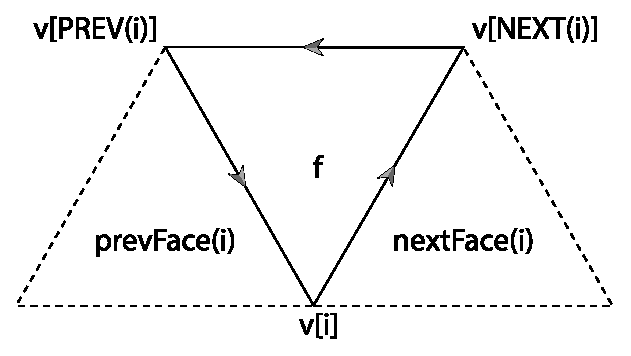
\includegraphics[width=0.4\linewidth]{chap03/Subdivprevnextface.eps}
    \caption{给定顶点{\ttfamily\refvar[SDFace::v]{v}{}[i]}和附带的面{\ttfamily f},
    我们定义\emph{下一面}为与{\ttfamily f}通过
    从{\ttfamily\protect\refvar[SDFace::v]{v}{}[i]}到{\ttfamily\protect\refvar[SDFace::v]{v}{}[\protect\refvar{NEXT}{}(i)]}的边邻接的面。
    上一面的定义类似。}
    \label{fig:3.29}
\end{figure}

通过依次转到围绕\refvar[SDFace::v]{v}{}的下一面,
我们可以遍历与之相邻的面
\sidenote{译者注:思考一下,相容次序为这种遍历提供了什么便利?}。
如果我们最终回到出发的面,则我们位于内部顶点上;
如果我们遇到一条边的相邻指针是{\ttfamily nullptr},
则我们位于边界顶点上(\reffig{3.30})。
一旦初始化例程确定这是否是边界顶点,
它就计算顶点的价,如果是价为6的内部顶点或价为4的边界顶点,
就置位标志\refvar{regular}{};否则这是个非凡顶点。
\begin{figure}[htbp]
    \centering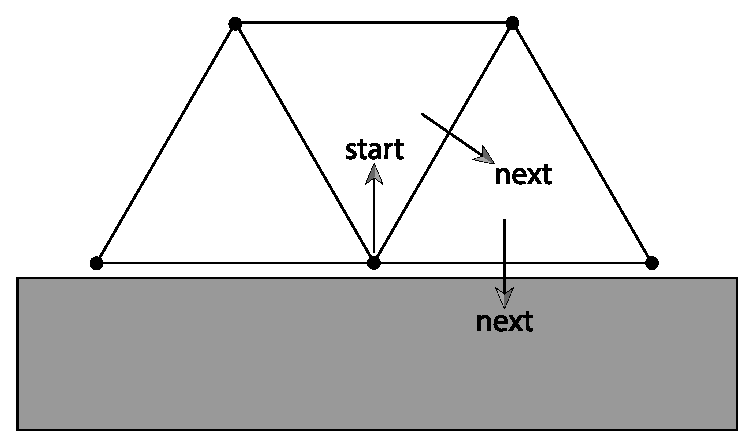
\includegraphics[width=0.5\linewidth]{chap03/Subdivdetermineboundary.eps}
    \caption{我们可以通过从相邻面\protect\refvar{startFace}{}开始
        并跟随围绕该顶点的下一面指针来确定一个顶点是否是边界顶点。
        如果我们遇到一个没有下一相邻面的面,则该顶点在边界上。
        如果我们回到\protect\refvar{startFace}{},则它是内部顶点。}
    \label{fig:3.30}
\end{figure}

\begin{lstlisting}
`\initcode{Finish vertex initialization}{=}`
for (int i = 0; i < nVertices; ++i) {
    `\refvar{SDVertex}{}` *v = vertices[i];
    `\refvar{SDFace}{}` *f = v->`\refvar{startFace}{}`;
    do {
        f = f->`\refvar{nextFace}{}`(v);
    } while (f && f != v->`\refvar{startFace}{}`);
    v->`\refvar[SDVertex::boundary]{boundary}{}` = (f == nullptr);
    if (!v->`\refvar[SDVertex::boundary]{boundary}{}` && v->`\refvar{valence}{}`() == 6)
        v->`\refvar{regular}{}` = true;
    else if (v->`\refvar[SDVertex::boundary]{boundary}{}` && v->`\refvar{valence}{}`() == 4)
        v->`\refvar{regular}{}` = true;
    else
        v->`\refvar{regular}{}` = false;
}
\end{lstlisting}

因为经常需要顶点的价,所以我们提供方法\refvar[valence]{SDVertex::valence}{()}
\sidenote{译者注:我认为该方法可能不适合处理一些极其特殊罕见的情况,
    但确实够用了,详见\url{https://github.com/mmp/pbrt-v4/issues/143}。}。
\begin{lstlisting}
`\initcode{LoopSubdiv Inline Functions}{=}\initnext{LoopSubdivInlineFunctions}`
inline int `\refvar{SDVertex}{}`::`\initvar{valence}{}`() {
    `\refvar{SDFace}{}` *f = `\refvar{startFace}{}`;
    if (!`\refvar[SDVertex::boundary]{boundary}{}`) {
        `\refcode{Compute valence of interior vertex}{}`
    } else {
        `\refcode{Compute valence of boundary vertex}{}`
    }
}
\end{lstlisting}

为了计算非边界顶点的价,该方法跟随每个面围绕该顶点的相邻指针
开始计算相邻面的数量,直到它回到出发的面。
价等于访问的面的数量。
\begin{lstlisting}
`\initcode{Compute valence of interior vertex}{=}`
int nf = 1;
while ((f = f->`\refvar{nextFace}{}`(this)) != `\refvar{startFace}{}`)
    ++nf;
return nf;
\end{lstlisting}

对于边界顶点我们可以用相同的方法,但这种情况下价比相邻面的数量多一。
这里遍历相邻面稍微更复杂些:它跟随围绕该顶点的下一面指针直到遇到边界,计算见过的面的数量。
然后它再次从\refvar{startFace}{}开始并跟随上一面指针直到在另一方向遇到边界。
\begin{lstlisting}
`\initcode{Compute valence of boundary vertex}{=}`
int nf = 1;
while ((f = f->`\refvar{nextFace}{}`(this)) != nullptr)
    ++nf;
f = `\refvar{startFace}{}`;
while ((f = f->`\refvar{prevFace}{}`(this)) != nullptr)
    ++nf;
return nf + 1;
\end{lstlisting}

\refvar[vnum]{SDFace::vnum}{()}是查找给定顶点指针的索引的实用函数。
传入一个不属于当前的面的顶点指针是致命错误——
这种情况表明细分代码中有bug。
\begin{lstlisting}
`\initcode{SDFace Methods}{=}\initnext{SDFaceMethods}`
int `\initvar{vnum}{}`(`\refvar{SDVertex}{}` *vert) const {
    for (int i = 0; i < 3; ++i)
        if (`\refvar[SDFace::v]{v}{}`[i] == vert) return i;
    `\refvar{Severe}{}`("Basic logic error in SDFace::vnum()");
    return -1;
}
\end{lstlisting}

因为面{\ttfamily f}上顶点{\ttfamily\refvar[SDFace::v]{v}{}[i]}的
下一面在第i边上(回想\reffig{3.27}中相邻边指针的映射),
给定实用函数\refvar{vnum}{()}提供的顶点索引{\ttfamily i},
我们可轻松找出合适的相邻面指针。
上一面邻接从{\ttfamily\refvar{PREV}{}(i)}到{\ttfamily i}的边,
所以对于上一面该方法返回{\ttfamily \refvar[SDFace::f]{f}{}[\refvar{PREV}{}(i)]}。
\begin{lstlisting}
`\refcode{SDFace Methods}{+=}\lastnext{SDFaceMethods}`
`\refvar{SDFace}{}` *`\initvar{nextFace}{}`(`\refvar{SDVertex}{}` *vert) {
    return `\refvar[SDFace::f]{f}{}`[`\refvar{vnum}{}`(vert)];
}
\end{lstlisting}
\begin{lstlisting}
`\refcode{SDFace Methods}{+=}\lastnext{SDFaceMethods}`
`\refvar{SDFace}{}` *`\initvar{prevFace}{}`(`\refvar{SDVertex}{}` *vert) {
    return `\refvar[SDFace::f]{f}{}`[`\refvar{PREV}{}`(`\refvar{vnum}{}`(vert))];
}
\end{lstlisting}

能够从任意顶点开始获取围绕一个面的上一个和下一个顶点也很有用。
方法\refvar[nextVert]{SDFace::nextVert}{()}和\refvar[prevVert]{SDFace::prevVert}{()}就是干这个的(\reffig{3.31})。
\begin{figure}[htbp]
    \centering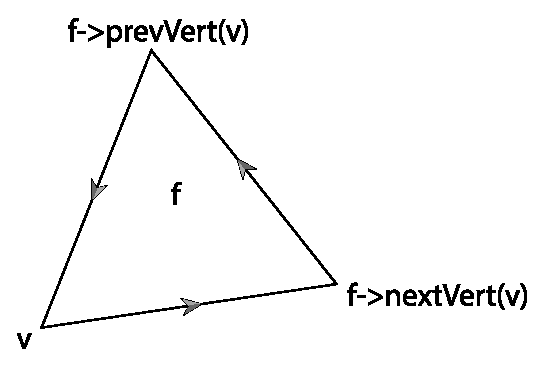
\includegraphics[width=0.35\linewidth]{chap03/Subdivprevnextvert.eps}
    \caption{给定顶点{\ttfamily v}和面{\ttfamily f},
    方法{\ttfamily f->\protect\refvar{prevVert}{}(v)}返回
    从{\ttfamily v}起绕该面的上一个顶点,
    而{\ttfamily f->\protect\refvar{nextVert}{}(v)}返回下一个顶点,
    其中“下一个”和“上一个”由定义该面时的顶点原始顺序定义。}
    \label{fig:3.31}
\end{figure}

\begin{lstlisting}
`\refcode{SDFace Methods}{+=}\lastnext{SDFaceMethods}`
`\refvar{SDVertex}{}` *`\initvar{nextVert}{}`(`\refvar{SDVertex}{}` *vert) {
    return `\refvar[SDFace::v]{v}{}`[`\refvar{NEXT}{}`(`\refvar{vnum}{}`(vert))];
}
\end{lstlisting}
\begin{lstlisting}
`\refcode{SDFace Methods}{+=}\lastnext{SDFaceMethods}`
`\refvar{SDVertex}{}` *`\initvar{prevVert}{}`(`\refvar{SDVertex}{}` *vert) {
    return `\refvar[SDFace::v]{v}{}`[`\refvar{PREV}{}`(`\refvar{vnum}{}`(vert))];
}
\end{lstlisting}

\subsection{细分}\label{sub:细分}
现在我们可以展示怎样用修改后的Loop规则进行细分了。
这里的实现施加固定次数的细分来为渲染生成三角网格;
本章末习题7讨论了自适应细分,每个原始面都被细分足够的次数
使得从特定视点观察的结果是光滑的,而不是仅用固定层级数的细分,
否则一些区域可能过细分而同时另一些则欠细分。

代码片\refcode{Refine subdivision mesh into triangles}{}反复
对网格运用细分规则,每次都生成一个新网格用作下一步的输入。
每次细分步骤后,数组{\ttfamily f}和{\ttfamily v}都更新为
指向来自刚完成的细分层级的面和顶点。
当细分完成时,便返回曲面的三角网格表示。

类\refvar{MemoryArena}{}的实例用于在该过程中分配临时存储。
该类定义于\refsub{基于Arena的分配},提供了快速的自定义内存分配方法,
当它离开作用域时会自动释放内存。

\begin{lstlisting}
`\initcode{Refine subdivision mesh into triangles}{=}`
std::vector<`\refvar{SDFace}{}` *> f = faces;
std::vector<`\refvar{SDVertex}{}` *> v = vertices;
`\refvar{MemoryArena}{}` arena;
for (int i = 0; i < nLevels; ++i) {
    `\refcode{Update f and v for next level of subdivision}{}`
}
`\refcode{Push vertices to limit surface}{}`
`\refcode{Compute vertex tangents on limit surface}{}`
`\refcode{Create triangle mesh from subdivision mesh}{}`
\end{lstlisting}

细分步骤主循环的过程如下:它创建{\ttfamily vector}来存储
当前细分层级的顶点和面,并继续计算新顶点位置,更新细化网格的拓扑表示。
\reffig{3.32}展示了网格中面的基本细化规则。
每个面被分为四个子面,第{\ttfamily i}个子面
与输入面的第{\ttfamily i}个顶点相邻且最后一个面位于中心。
然后沿原始面的分割边计算三个新顶点。
\begin{figure}[htbp]
    \centering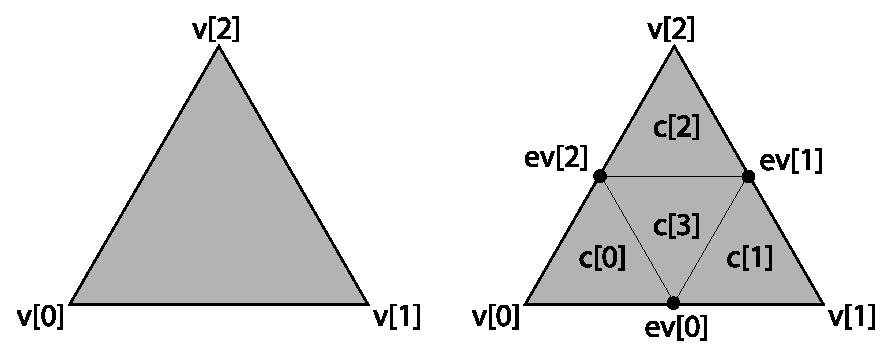
\includegraphics[width=0.6\linewidth]{chap03/Subdivrefinementnaming.eps}
    \caption{单个三角面的基本细分。创建和排序四个子面,第{\ttfamily i}个子面
    与原始面的第{\ttfamily i}个顶点相邻且第四个子面位于细分面的中心。
    需要计算三条边上的顶点;它们的编号满足第{\ttfamily i}个边上顶点在原始面的第{\ttfamily i}条边上。}
    \label{fig:3.32}
\end{figure}

\begin{lstlisting}
`\initcode{Update f and v for next level of subdivision}{=}`
std::vector<`\refvar{SDFace}{}` *> newFaces;
std::vector<`\refvar{SDVertex}{}` *> newVertices;
`\refcode{Allocate next level of children in mesh tree}{}`
`\refcode{Update vertex positions and create new edge vertices}{}`
`\refcode{Update new mesh topology}{}`
`\refcode{Prepare for next level of subdivision}{}`
\end{lstlisting}

首先,为已经出现在输入网格中的顶点的更新值分配存储。该方法还为子面分配存储。
但除了设置顶点的标志\refvar{regular}{}和\refvar[SDVertex::boundary]{boundary}{}外,
它还没对新顶点和面做任何初始化,因为细分让边界顶点仍在边界上,
内部顶点仍在内部,且不改变网格中顶点的价。
\begin{lstlisting}
`\initcode{Allocate next level of children in mesh tree}{=}`
for (`\refvar{SDVertex}{}` *vertex : v) {
    vertex->`\refvar{child}{}` = arena.`\refvar[MemoryArena:Alloc2]{Alloc}{}`<`\refvar{SDVertex}{}`>();
    vertex->`\refvar{child}{}`->`\refvar{regular}{}` = vertex->`\refvar{regular}{}`;
    vertex->`\refvar{child}{}`->`\refvar[SDVertex::boundary]{boundary}{}` = vertex->`\refvar[SDVertex::boundary]{boundary}{}`;
    newVertices.push_back(vertex->`\refvar{child}{}`);
}
for (`\refvar{SDFace}{}` *face : f) {
    for (int k = 0; k < 4; ++k) {
        face->`\refvar{children}{}`[k] = arena.`\refvar[MemoryArena:Alloc2]{Alloc}{}`<`\refvar{SDFace}{}`>();
        newFaces.push_back(face->`\refvar{children}{}`[k]);
    }
}
\end{lstlisting}

\subsubsection*{计算新顶点的位置}
在担心细分网格的拓扑初始化之前,细化方法先为网格中的所有顶点计算位置。
首先,它考虑所有已经出现于网格中的顶点的更新位置计算问题;
这些顶点称为\keyindex{偶顶点}{even vertex}{vertex顶点}。
然后它计算分割边上的新顶点,称为\keyindex{奇顶点}{odd vertex}{vertex顶点}。
\begin{lstlisting}
`\initcode{Update vertex positions and create new edge vertices}{=}`
`\refcode{Update vertex positions for even vertices}{}`
`\refcode{Compute new odd edge vertices}{}`
\end{lstlisting}

对于偶顶点的每种不同类型——正则与非凡、边界与内部,
计算更新位置使用的技术不同。这给出了四种要处理的情况。
\begin{lstlisting}
`\initcode{Update vertex positions for even vertices}{=}`
for (`\refvar{SDVertex}{}` *vertex : v) {
    if (!vertex->`\refvar[SDVertex::boundary]{boundary}{}`) {
        `\refcode{Apply one-ring rule for even vertex}{}`
    } else {
        `\refcode{Apply boundary rule for even vertex}{}`
    }
}
\end{lstlisting}

对于内部顶点的两种类型,我们取每个顶点的相邻顶点集合
(称为绕它的\keyindex{一环}{one-ring}{},反映了它是一圈邻居的事实)
并用权重$\beta$为每个邻居顶点赋权(\reffig{3.33})。
我们正在更新的中心顶点赋权为$1-n\beta$,其中$n$为该顶点的价。
因此,顶点$\bm v$对应的新顶点$\bm v'$为
\begin{align*}
    \bm v'=(1-n\beta)\bm v+\sum\limits_{i=1}^{N}{\beta \bm v_i}\, .
\end{align*}

该公式确保权重之和为一,保证了Loop细分曲面的凸包性质,
确保最终网格在控制网格的凸包内。
正在更新的顶点位置只受附近顶点的影响;
这称为\keyindex{局部支撑}{local support}{}。
Loop细分尤其高效,因为其细分规则均有该性质。
\begin{figure}[htbp]
    \centering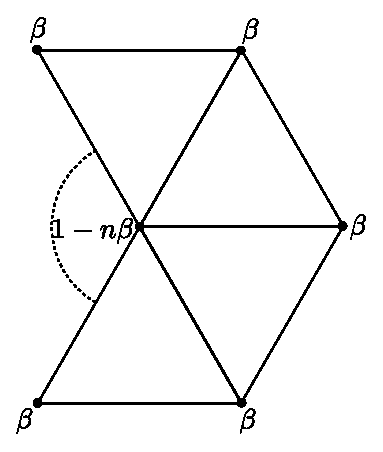
\includegraphics[width=0.3\linewidth]{chap03/Subdivoneringweighting.eps}
    \caption{顶点$\bm v$的新顶点$\bm v'$通过用权重$\beta$对相邻顶点$\bm v_i$赋权、
        用$(1-n\beta)$对$\bm v$赋权计算得到,其中$n$为$\bm v$的价。
        相邻顶点$\bm v_i$统称为绕$\bm v$的\emph{一环}。}
    \label{fig:3.33}
\end{figure}

该步骤所用的指定权重$\beta$是细分方法的关键组成,
必须仔细选取以保证极限曲面的光滑性以及其他所需的性质
\footnote{再次见本节开头和“扩展阅读”一节引用的文献
    了解关于如何推导出$\beta$等值的信息。}。
下面的函数\refvar{beta}{()}基于顶点的价计算能够保证光滑性的$\beta$值。
对于正则内部顶点,\refvar{beta}{()}返回$\displaystyle\frac{1}{16}$。
因为这是常见情况,所以实现直接用$\displaystyle\frac{1}{16}$而不是每次都调用\refvar{beta}{()}。
\begin{lstlisting}
`\initcode{Apply one-ring rule for even vertex}{=}`
if (vertex->`\refvar{regular}{}`)
    vertex->`\refvar{child}{}`->`\refvar[SDVertex::p]{p}{}` = `\refvar{weightOneRing}{}`(vertex, 1.f / 16.f);
else
    vertex->`\refvar{child}{}`->`\refvar[SDVertex::p]{p}{}` = `\refvar{weightOneRing}{}`(vertex, `\refvar{beta}{}`(vertex->`\refvar{valence}{}`()));
\end{lstlisting}
\begin{lstlisting}
`\refcode{LoopSubdiv Inline Functions}{+=}\lastnext{LoopSubdivInlineFunctions}`
inline `\refvar{Float}{}` `\initvar{beta}{}`(int valence) {
    if (valence == 3) return 3.f / 16.f;
    else return 3.f / (8.f * valence);
}
\end{lstlisting}

函数\refvar{weightOneRing}{()}遍历一环相邻顶点并用给定权重计算新顶点位置。
它用后面定义的方法\refvar[oneRing]{SDVertex::oneRing}{()}
返回绕顶点{\ttfamily vert}的顶点位置。
\begin{lstlisting}
`\refcode{LoopSubdiv Function Definitions}{+=}\lastnext{LoopSubdivFunctionDefinitions}`
static `\refvar{Point3f}{}` `\initvar{weightOneRing}{}`(`\refvar{SDVertex}{}` *vert, `\refvar{Float}{}` beta) {
    `\refcode{Put vert one-ring in pRing}{}`
    `\refvar{Point3f}{}` p = (1 - valence * beta) * vert->`\refvar[SDVertex::p]{p}{}`;
    for (int i = 0; i < valence; ++i)
        p += beta * pRing[i];
    return p;
}  
\end{lstlisting}

因为一环内有不定数量的顶点,所以我们用宏\refvar{ALLOCA}{()}来
高效分配空间存储它们的位置。
\begin{lstlisting}
`\initcode{Put vert one-ring in pRing}{=}`
int valence = vert->`\refvar{valence}{}`();
`\refvar{Point3f}{}` *pRing = `\refvar{ALLOCA}{}`(`\refvar{Point3f}{}`, valence);
vert->`\refvar{oneRing}{}`(pRing);
\end{lstlisting}

方法\refvar{oneRing}{()}假设传入的指针指向一片足够大的内存区域以存储绕该顶点的一环。
\begin{lstlisting}
`\refcode{LoopSubdiv Function Definitions}{+=}\lastnext{LoopSubdivFunctionDefinitions}`
void `\refvar{SDVertex}{}`::`\initvar{oneRing}{}`(`\refvar{Point3f}{}` *p) {
    if (!`\refvar[SDVertex::boundary]{boundary}{}`) {
        `\refcode{Get one-ring vertices for interior vertex}{}`
    } else {
        `\refcode{Get one-ring vertices for boundary vertex}{}`
    }
}
\end{lstlisting}

获取绕内部顶点的一环相对简单,可以通过遍历与该顶点相邻的面并
对每个面保留中心顶点后面的那个顶点来实现
(用笔纸简单打个草稿你就能理解该过程会返回一环内的所有顶点)。
\begin{lstlisting}
`\initcode{Get one-ring vertices for interior vertex}{=}`
`\refvar{SDFace}{}` *face = `\refvar{startFace}{}`;
do {
    *p++ = face->`\refvar{nextVert}{}`(this)->`\refvar[SDVertex::p]{p}{}`;
    face = face-`\refvar{nextFace}{}`(this);
} while (face != `\refvar{startFace}{}`);
\end{lstlisting}

绕边界顶点的一环有些棘手。
这里的实现在给定的\refvar{Point3f}{}数组中仔细存储一环,
使数组中首尾元素是沿边界的相邻顶点。
该顺序很重要,因为相邻边界顶点的赋权常常不同于网格内部的相邻顶点。
这样做要求我们先遍历周围相邻面直到到达边界,
然后朝另一个方向遍历,并一个接一个地存储顶点。
\begin{lstlisting}
`\initcode{Get one-ring vertices for boundary vertex}{=}`
`\refvar{SDFace}{}` *face = `\refvar{startFace}{}`, *f2;
while ((f2 = face->`\refvar{nextFace}{}`(this)) != nullptr)
    face = f2;
*p++ = face->`\refvar{nextVert}{}`(this)->`\refvar[SDVertex::p]{p}{}`;
do {
    *p++ = face->`\refvar{prevVert}{}`(this)->`\refvar[SDVertex::p]{p}{}`;
    face = face->`\refvar{prevFace}{}`(this);
} while (face != nullptr);
\end{lstlisting}

对于边界上的顶点,新顶点的位置只基于两个邻接边界顶点(\reffig{3.34})。
不依赖内部顶点保证了共享着边界上相同顶点的
两个邻接\sidenote{译者注:原文abutting。}曲面会有邻接的极限曲面。
实用函数\refvar{weightBoundary}{()}将给定权重赋给
两个相邻顶点$\bm v_1$和$\bm v_2$来算得新位置$\bm v'$为
\begin{align*}
    \bm v'=(1-2\beta)\bm v+\beta\bm v_1+\beta\bm v_2\, .
\end{align*}

正则和非凡顶点都用相同的权重$\displaystyle\frac{1}{8}$。
\begin{figure}[htbp]
    \centering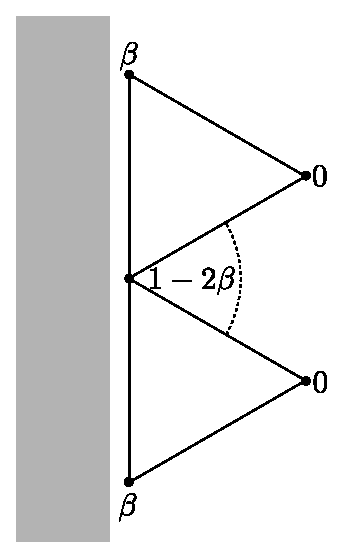
\includegraphics[width=0.25\linewidth]{chap03/Subdivboundaryweighting.eps}
    \caption{边界边上的细分。中心顶点的新位置通过对它和它的两个相邻顶点赋予所示权重算得。}
    \label{fig:3.34}
\end{figure}

\begin{lstlisting}
`\initcode{Apply boundary rule for even vertex}{=}`
vertex->`\refvar{child}{}`->`\refvar[SDVertex::p]{p}{}` = `\refvar{weightBoundary}{}`(vertex, 1.f / 8.f);
\end{lstlisting}

实用函数\refvar{weightBoundary}{()}将给定权重赋给边界顶点。
它的实现很简单,因为函数\refvar[oneRing]{SDVertex::oneRing}{()}将
边界顶点的一环排成首尾元素是边界邻居。
\begin{lstlisting}
`\refcode{LoopSubdiv Function Definitions}{+=}\lastcode{LoopSubdivFunctionDefinitions}`
static `\refvar{Point3f}{}` `\initvar{weightBoundary}{}`(`\refvar{SDVertex}{}` *vert, `\refvar{Float}{}` beta) {
    `\refcode{Put vert one-ring in pRing}{}`
    `\refvar{Point3f}{}` p = (1 - 2 * beta) * vert->`\refvar[SDVertex::p]{p}{}`;
    p += beta * pRing[0];
    p += beta * pRing[valence - 1];
    return p;
}
\end{lstlisting}

现在细化方法计算奇顶点的位置——沿网格分割边的新顶点。
它遍历网格中每个面的每条边,计算划分边的新顶点(\reffig{3.35})。
对于内部边,通过赋权边两端的顶点以及
该边相邻面的相对顶点可以求得新顶点。
它遍历每个面的全部三条边,每次遇到之前没见过的边它就
计算对应该边的新的奇顶点并存于关联的{\ttfamily edgeVerts}数组中。
\begin{figure}[htbp]
    \centering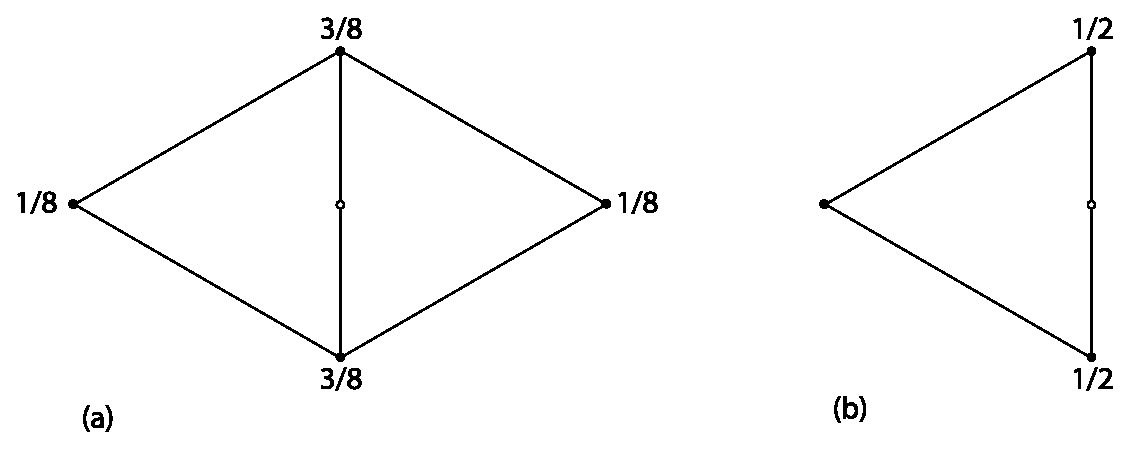
\includegraphics[width=0.75\linewidth]{chap03/Subdivedgesplit.eps}
    \caption{边分割的细分规则。空心圆标出的新的奇顶点的位置是通过
        赋权该边两端的顶点以及相邻三角形与之相对的两个顶点求得的。
        (a)内部顶点的权重;(b)边界顶点的权重。}
    \label{fig:3.35}
\end{figure}

\begin{lstlisting}
`\initcode{Compute new odd edge vertices}{=}`
std::map<`\refvar{SDEdge}{}`, `\refvar{SDVertex}{}` *> edgeVerts;
for (`\refvar{SDFace}{}` *face : f) {
    for (int k = 0; k < 3; ++k) {
        `\refcode{Compute odd vertex on kth edge}{}`
    }
}
\end{lstlisting}

就像设置原始网格中的相邻面指针做的那样,
为每条边创建\refvar{SDEdge}{}对象并检查它是否在已访问的边集合中。
如果没在,则计算该边上的新顶点并添入{\ttfamily map},
它是高效执行查找的关联数组结构。
\begin{lstlisting}
`\initcode{Compute odd vertex on kth edge}{=}`
`\refvar{SDEdge}{}` edge(face->`\refvar[SDFace::v]{v}{}`[k], face->`\refvar[SDFace::v]{v}{}`[`\refvar{NEXT}{}`(k)]);
`\refvar{SDVertex}{}` *vert = edgeVerts[edge];
if (!vert) {
    `\refcode{Create and initialize new odd vertex}{}`
    `\refcode{Apply edge rules to compute new vertex position}{}`
    edgeVerts[edge] = vert;
}
\end{lstlisting}

在Loop细分中,细分加入的新顶点总是正则的
(这意味着非凡顶点相对于正则顶点的比例会随着每级细分下降)。
因此,新顶点的成员\refvar{regular}{}可以立即设为{\ttfamily true}。
成员\refvar[SDVertex::boundary]{boundary}{}也很容易通过检查正在分割的边是否有相邻面来初始化。
最后,新顶点的指针\refvar{startFace}{}也可在这里设置。
对于一个面的边上任何一个奇顶点,中心孩子(三号子面)保证与新顶点相邻。
\begin{lstlisting}
`\initcode{Create and initialize new odd vertex}{=}`
vert = arena.`\refvar[MemoryArena:Alloc2]{Alloc}{}`<`\refvar{SDVertex}{}`>();
newVertices.push_back(vert);
vert->`\refvar{regular}{}` = true;
vert->`\refvar[SDVertex::boundary]{boundary}{}` = (face->`\refvar[SDFace::f]{f}{}`[k] == nullptr);
vert->`\refvar{startFace}{}` = face->`\refvar{children}{}`[3];
\end{lstlisting}

对于边界奇顶点,新顶点只是两个相邻顶点的均值。
对于内部奇顶点,该边两端顶点被赋权$\displaystyle\frac{3}{8}$,
与该边相对的两个顶点被赋权$\displaystyle\frac{1}{8}$(\reffig{3.35})。
后两个顶点可用实用函数\refvar[otherVert]{SDFace::otherVert}{()}找到,
返回一个面与给定边相对的顶点。
\begin{lstlisting}
`\initcode{Apply edge rules to compute new vertex position}{=}`
if (vert->`\refvar[SDVertex::boundary]{boundary}{}`) {
    vert->`\refvar[SDVertex::p]{p}{}` =  0.5f * edge.`\refvar[SDEdge::v]{v}{}`[0]->`\refvar[SDVertex::p]{p}{}`;
    vert->`\refvar[SDVertex::p]{p}{}` += 0.5f * edge.`\refvar[SDEdge::v]{v}{}`[1]->`\refvar[SDVertex::p]{p}{}`;
} else {
    vert->`\refvar[SDVertex::p]{p}{}` =  3.f/8.f * edge.`\refvar[SDEdge::v]{v}{}`[0]->`\refvar[SDVertex::p]{p}{}`;
    vert->`\refvar[SDVertex::p]{p}{}` += 3.f/8.f * edge.`\refvar[SDEdge::v]{v}{}`[1]->`\refvar[SDVertex::p]{p}{}`;
    vert->`\refvar[SDVertex::p]{p}{}` += 1.f/8.f * face->`\refvar{otherVert}{}`(edge.`\refvar[SDEdge::v]{v}{}`[0], edge.`\refvar[SDEdge::v]{v}{}`[1])->`\refvar[SDVertex::p]{p}{}`;
    vert->`\refvar[SDVertex::p]{p}{}` += 1.f/8.f *
        face->`\refvar[SDFace::f]{f}{}`[k]->`\refvar{otherVert}{}`(edge.`\refvar[SDEdge::v]{v}{}`[0], edge.`\refvar[SDEdge::v]{v}{}`[1])->`\refvar[SDVertex::p]{p}{}`;
}
\end{lstlisting}

方法\refvar[otherVert]{SDFace::otherVert}{()}不言自明
\sidenote{译者注:我认为第6行提示有些不准确,已修改。详见\url{https://github.com/mmp/pbrt-v4/issues/146}。}:
\begin{lstlisting}
`\refcode{SDFace Methods}{+=}\lastcode{SDFaceMethods}`
`\refvar{SDVertex}{}` *`\initvar{otherVert}{}`(`\refvar{SDVertex}{}` *v0, `\refvar{SDVertex}{}` *v1) {
    for (int i = 0; i < 3; ++i)
        if (`\refvar[SDFace::v]{v}{}`[i] != v0 && `\refvar[SDFace::v]{v}{}`[i] != v1)
            return `\refvar[SDFace::v]{v}{}`[i];
    `\refvar{Severe}{}`("Basic logic error in SDFace::otherVert()");
    return nullptr;
}
\end{lstlisting}

\subsubsection*{更新网格拓扑}
为了让拓扑更新的细节尽可能简单,
仔细选取细分面及其顶点的编号方案(\reffig{3.36})。
仔细看图;所示约定是后面几页的关键。
\begin{figure}[htbp]
    \centering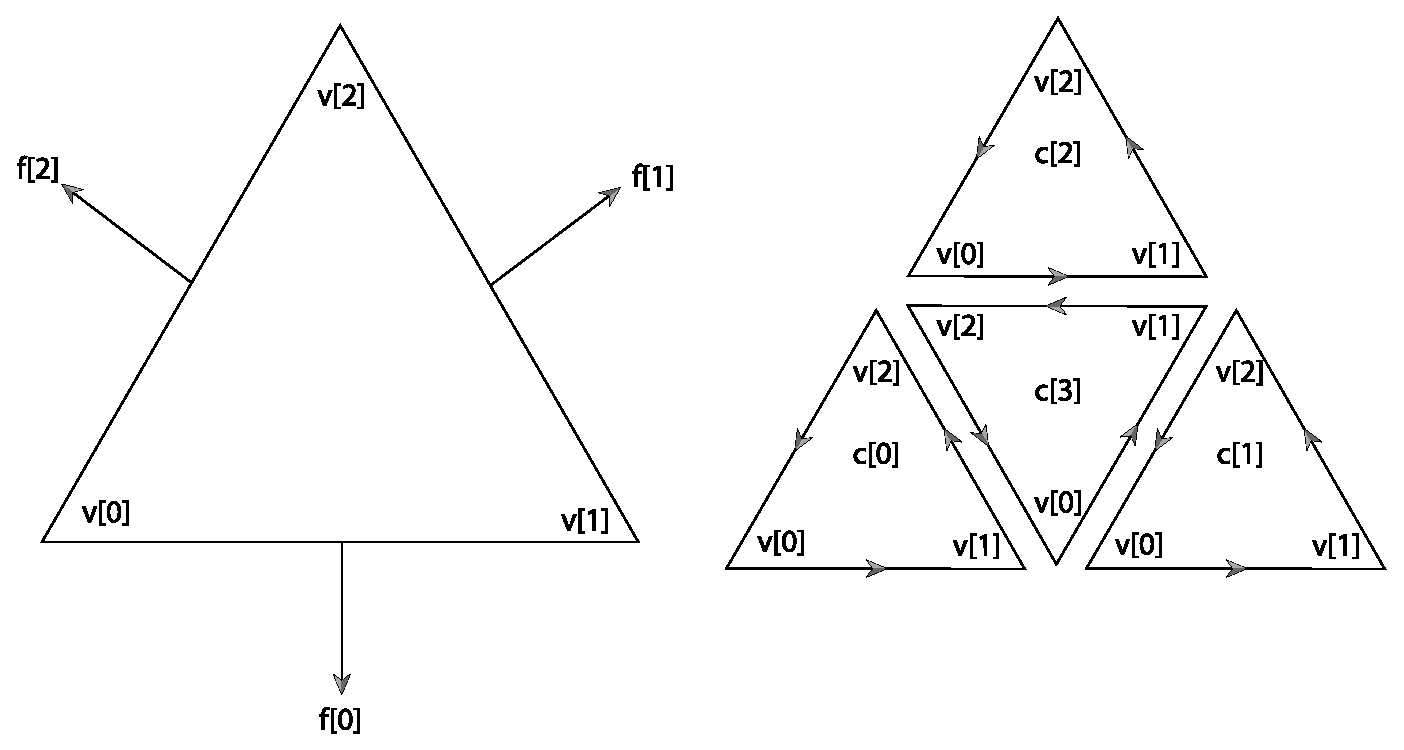
\includegraphics[width=\linewidth]{chap03/Subdivvertfacepointerupdate.eps}
    \caption{每个面都分为四个子面,第{\ttfamily i}子面与原始面的第{\ttfamily i}顶点相邻,
    第{\ttfamily i}子面的第{\ttfamily i}顶点是原始面的第{\ttfamily i}顶点。
    中心子面的顶点朝向为第{\ttfamily i}顶点是沿父面第{\ttfamily i}边的奇顶点。}
    \label{fig:3.36}
\end{figure}

更新细化网格的拓扑指针需要四大任务:
\begin{enumerate}
    \item 奇顶点的指针\refvar[startFace]{SDVertex::startFace}{}需存储指向其相邻面之一的指针。
    \item 同样,必须设置偶顶点的指针\refvar[startFace]{SDVertex::startFace}{}。
    \item 需要设置新面的相邻指针{\ttfamily\refvar[SDFace::f]{f}{}[i]}指向相邻面。
    \item 新面的指针{\ttfamily\refvar[SDFace::v]{v}{}[i]}需要指向合适的顶点。
\end{enumerate}

奇顶点的指针\refvar{startFace}{}在首次创建时就已经初始化了。
这里我们依次处理其余三个任务。
\begin{lstlisting}
`\initcode{Update new mesh topology}{=}`
`\refcode{Update even vertex face pointers}{}`
`\refcode{Update face neighbor pointers}{}`
`\refcode{Update face vertex pointers}{}`
\end{lstlisting}

如果一个顶点是其\refvar{startFace}{}的第{\ttfamily i}顶点,
则它保证会与\refvar{startFace}{}的第{\ttfamily i}子面相邻。
因此,只需要遍历网格中所有父顶点,
对每一个求取它在其\refvar{startFace}{}中的顶点索引。
然后可用该索引找到与新的偶顶点相邻的子面。
\begin{lstlisting}
`\initcode{Update even vertex face pointers}{=}`
for (`\refvar{SDVertex}{}` *vertex : v) {
    int vertNum = vertex->`\refvar{startFace}{}`->`\refvar{vnum}{}`(vertex);
    vertex->`\refvar{child}{}`->`\refvar{startFace}{}` = 
        vertex->`\refvar{startFace}{}`->`\refvar{children}{}`[vertNum];
}
\end{lstlisting}

接着,更新新建面的相邻面指针。
我们将其分为两步:一个是更新同父的子面间的邻居,
一个是更新异父的子面间的邻居。这涉及一些棘手的指针操作。
\begin{lstlisting}
`\initcode{Update face neighbor pointers}{=}`
for (`\refvar{SDFace}{}` *face : f) {
    for (int j = 0; j < 3; ++j) {
        `\refcode{Update children f pointers for siblings}{}`
        `\refcode{Update children f pointers for neighbor children}{}`
    }
}
\end{lstlisting}

对于第一步,回想内部子面总是存于{\ttfamily\refvar{children}{}[3]}。
而且(对于{\ttfamily k}=0,1,2)第{\ttfamily k+1}子面相邻于内部面的第{\ttfamily k}边,
内部面相邻于第{\ttfamily k}面的第{\ttfamily k+1}边。
\begin{lstlisting}
`\initcode{Update children f pointers for siblings}{=}`
face->`\refvar{children}{}`[3]->`\refvar[SDFace::f]{f}{}`[j] = face->`\refvar{children}{}`[`\refvar{NEXT}{}`(j)];
face->`\refvar{children}{}`[j]->`\refvar[SDFace::f]{f}{}`[`\refvar{NEXT}{}`(j)] = face->`\refvar{children}{}`[3];
\end{lstlisting}

我们现在更新子面的指向其他父亲之子的相邻指针。
这里只有前三个子面需要处理;内部子面的相邻指针已经完全初始化了。
观察\reffig{3.36}可知第{\ttfamily k}个子面
\sidenote{译者注:原文写为第{\ttfamily i}个子面,我认为是笔误,此处已修正。}需要设置
第{\ttfamily k}和{\ttfamily\refvar{PREV}{}(k)}边。
为了设置第{\ttfamily k}子面的第{\ttfamily k}边,
我们先求父面的第{\ttfamily k}边,
则相邻父面{\ttfamily f2}与那条边相邻。
若{\ttfamily f2}存在(意味着我们不在边界上),
则求得顶点{\ttfamily v[k]}的相邻父索引。
该索引等于我们正在搜索的相邻子面的索引。
然后重复该过程寻找与第{\ttfamily\refvar{PREV}{}(k)}边相邻的子面。
\begin{lstlisting}
`\initcode{Update children f pointers for neighbor children}{=}`
`\refvar{SDFace}{}` *f2 = face->`\refvar[SDFace::f]{f}{}`[j];
face->`\refvar{children}{}`[j]->`\refvar[SDFace::f]{f}{}`[j] =
    f2 ? f2->`\refvar{children}{}`[f2->`\refvar{vnum}{}`(face->`\refvar[SDFace::v]{v}{}`[j])] : nullptr;
f2 = face->`\refvar[SDFace::f]{f}{}`[`\refvar{PREV}{}`(j)];
face->`\refvar{children}{}`[j]->`\refvar[SDFace::f]{f}{}`[`\refvar{PREV}{}`(j)] = 
    f2 ? f2->`\refvar{children}{}`[f2->`\refvar{vnum}{}`(face->`\refvar[SDFace::v]{v}{}`[j])] : nullptr;
\end{lstlisting}

最后,我们处理拓扑更新的第四步:设置子面的顶点指针。
\begin{lstlisting}
`\initcode{Update face vertex pointers}{=}`
for (`\refvar{SDFace}{}` *face : f) {
    for (int j = 0; j < 3; ++j) {
        `\refcode{Update child vertex pointer to new even vertex}{}`
        `\refcode{Update child vertex pointer to new odd vertex}{}`
    }
}
\end{lstlisting}

对于({\ttfamily k}=0,1,2)第{\ttfamily k}子面,
第{\ttfamily k}顶点对应于与该子面相邻的偶顶点。
对于非内部子面,有一个偶顶点和两个奇顶点;对于内部子面,有三个奇顶点。
通过跟随从父面获取的父顶点的子指针可以找到该顶点。
\begin{lstlisting}
`\initcode{Update child vertex pointer to new even vertex}{=}`
face->`\refvar{children}{}`[j]->`\refvar[SDFace::v]{v}{}`[j] = face->`\refvar[SDFace::v]{v}{}`[j]->`\refvar{child}{}`;
\end{lstlisting}

为了更新剩余顶点指针,再次用关联数组{\ttfamily edgeVerts}为父面的每条分割边寻找奇顶点。
三个子面以该顶点为事件\sidenote{译者注:原文incident。}顶点。
再次基于\reffig{3.36}中建立的编号方案,很容易求得该顶点在这三个面中的索引。
\begin{lstlisting}
`\initcode{Update child vertex pointer to new odd vertex}{=}`
`\refvar{SDVertex}{}` *vert = edgeVerts[`\refvar{SDEdge}{}`(face->`\refvar[SDFace::v]{v}{}`[j], face->`\refvar[SDFace::v]{v}{}`[`\refvar{NEXT}{}`(j)])];
face->`\refvar{children}{}`[j]->`\refvar[SDFace::v]{v}{}`[`\refvar{NEXT}{}`(j)] = vert;
face->`\refvar{children}{}`[`\refvar{NEXT}{}`(j)]->`\refvar[SDFace::v]{v}{}`[j] = vert;
face->`\refvar{children}{}`[3]->`\refvar[SDFace::v]{v}{}`[j] = vert;
\end{lstlisting}

一个细分步骤完成几何和拓扑工作后,
新建的顶点和面移入数组{\ttfamily v}和{\ttfamily f}:
\begin{lstlisting}
`\initcode{Prepare for next level of subdivision}{=}`
f = newFaces;
v = newVertices;
\end{lstlisting}

\subsubsection*{逼近极限曲面并输出}
细分曲面的显著性质之一是,如果我们永远继续细分下去,
特殊的细分规则可以给出网格顶点将有的位置。
这里我们用这些规则初始化极限曲面位置的数组{\ttfamily pLimit}。
注意计算中在顶点之外的地方临时存储极限曲面的位置很重要。
因为每个顶点的极限曲面位置依赖于其周围顶点的原始位置,
所有顶点的原始位置必须保持不变直到完成计算。

边界顶点的极限规则对两个相邻顶点赋权$\displaystyle\frac{1}{5}$,
中心顶点赋权$\displaystyle\frac{3}{5}$。
内部顶点的规则基于函数\refvar{loopGamma}{()},
它基于顶点的价计算合适的顶点权重。
\begin{lstlisting}
`\initcode{Push vertices to limit surface}{=}`
std::unique_ptr<`\refvar{Point3f}{}`[]> pLimit(new `\refvar{Point3f}{}`[v.size()]);
for (size_t i = 0; i < v.size(); ++i) {
    if (v[i]->`\refvar[SDVertex::boundary]{boundary}{}`)
        pLimit[i] =  `\refvar{weightBoundary}{}`(v[i], 1.f / 5.f);
    else
        pLimit[i] =  `\refvar{weightOneRing}{}`(v[i], `\refvar{loopGamma}{}`(v[i]->`\refvar{valence}{}`()));
}
for (size_t i = 0; i < v.size(); ++i)
    v[i]->`\refvar[SDVertex::p]{p}{}` = pLimit[i];
\end{lstlisting}
\begin{lstlisting}
`\refcode{LoopSubdiv Inline Functions}{+=}\lastcode{LoopSubdivInlineFunctions}`
inline `\refvar{Float}{}` `\initvar{loopGamma}{}`(int valence) {
    return 1.f / (valence + 3.f / (8.f * `\refvar{beta}{}`(valence)));
}
\end{lstlisting}

为了生成看起来光滑的、带有每个顶点曲面法线的三角网格,
每个顶点处都计算极限曲面一对不平行的切向量。
与位置的极限规则一样,这是给出实际极限曲面上精确切线的解析计算。
\begin{lstlisting}
`\initcode{Compute vertex tangents on limit surface}{=}`
std::vector<`\refvar{Normal3f}{}`> Ns;
Ns.reserve(v.size());
std::vector<`\refvar{Point3f}{}`> pRing(16, `\refvar{Point3f}{}`());
for (`\refvar{SDVertex}{}` *vertex : v) {
    `\refvar{Vector3f}{}` S(0,0,0), T(0,0,0);
    int valence = vertex->`\refvar{valence}{}`();
    if (valence > (int)pRing.size())
        pRing.resize(valence);
    vertex->`\refvar{oneRing}{}`(&pRing[0]);
    if (!vertex->`\refvar[SDVertex::boundary]{boundary}{}`) {
        `\refcode{Compute tangents of interior face}{}`
    } else {
        `\refcode{Compute tangents of boundary face}{}`
    }
    Ns.push_back(`\refvar{Normal3f}{}`(`\refvar{Cross}{}`(S, T)));
}
\end{lstlisting}

\reffig{3.37}展示了计算网格内部切线的设置。
中心顶点赋权为零,邻居赋权$w_i$。
\begin{figure}[htbp]
    \centering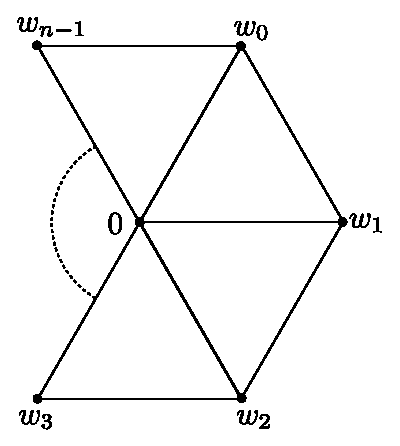
\includegraphics[width=0.35\linewidth]{chap03/Subdivtangents.eps}
    \caption{计算内部顶点的切线,一环顶点赋权为$w_i$。计算切线的中心顶点总是赋权为零。}
    \label{fig:3.37}
\end{figure}

为了计算首个切向量$\bm s$,权重为
\begin{align*}
    w_i=\cos{\left(\frac{2\pi i}{n}\right)}\, ,
\end{align*}
其中$n$为该顶点的价。计算第二个切向量$\bm t$用的权重为
\begin{align*}
    w_i=\sin{\left(\frac{2\pi i}{n}\right)}\, .
\end{align*}

\begin{lstlisting}
`\initcode{Compute tangents of interior face}{=}`
for (int j = 0; j < valence; ++j) {
    S += std::cos(2 * `\refvar{Pi}{}` * j / valence) * `\refvar{Vector3f}{}`(pRing[j]);
    T += std::sin(2 * `\refvar{Pi}{}` * j / valence) * `\refvar{Vector3f}{}`(pRing[j]);
}
\end{lstlisting}

边界顶点的切线有些棘手。\reffig{3.38}展示了后续讨论要求的一环顶点顺序
\sidenote{译者注:原图没有正确显示下标,已修正。}。
\begin{figure}[htbp]
    \centering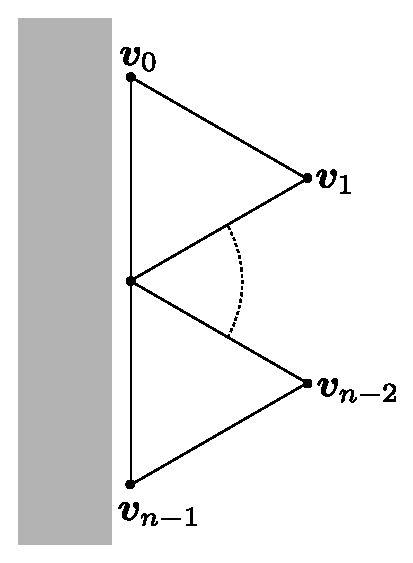
\includegraphics[width=0.35\linewidth]{chap03/Subdivedgetangents.eps}
    \caption{边界顶点的切线也计算为相邻顶点的加权平均。
        然而,一些边界切线规则并入了中心顶点的值。}
    \label{fig:3.38}
\end{figure}

第一条切线叫\keyindex{跨越切线}{across tangent}{tangent line切线},
由两相邻边界顶点间的向量给出:
\begin{align*}
    \bm s=\bm v_{n-1}-\bm v_0\, .
\end{align*}

第二条切线叫\keyindex{横断切线}{transverse tangent}{tangent line切线},
基于顶点的价算得。
中心顶点赋权$w_{\mathrm{c}}$,一环顶点赋权指定为向量$(w_0,w_1,\ldots,w_{n-1})$。
我们的横断切线规则是
\begin{table}[h]
    \centering\begin{tabular}{lll}
        \toprule
        价        & $w_{\mathrm{c}}$ & $w_i$       \\
        \midrule
        2         & -2               & (1,1)       \\
        3         & -1               & (0,1,0)     \\
        4(正则) & -2               & (-1,2,2,-1) \\
        \bottomrule
    \end{tabular}
\end{table}

价为5及以上时,$w_{\mathrm{c}}=0$且
\begin{align*}
    w_0 & =w_{n-1}=\sin{\theta}\, ,              \\
    w_i & =(2\cos{\theta}-2)\sin{(\theta i)}\, ,
\end{align*}
其中
\begin{align*}
    \theta=\frac{\pi}{n-1}\, .
\end{align*}

尽管这里我们没有证明,但对于所有$i$值这些权重都有和为零。
这保证了加权和实际上是切向量。
\begin{lstlisting}
`\initcode{Compute tangents of boundary face}{=}`
S = pRing[valence - 1] - pRing[0];
if (valence == 2)
    T = `\refvar{Vector3f}{}`(pRing[0] + pRing[1] - 2 * vertex->`\refvar[SDVertex::p]{p}{}`);
else if (valence == 3)
    T = pRing[1] - vertex->`\refvar[SDVertex::p]{p}{}`;
else if (valence == 4) // regular
    T = `\refvar{Vector3f}{}`(-1 * pRing[0] +  2 * pRing[1] + 2 * pRing[2] + 
                 -1 * pRing[3] + -2 * vertex->`\refvar[SDVertex::p]{p}{}`);
else {
    `\refvar{Float}{}` theta = `\refvar{Pi}{}` / float(valence - 1);
    T = `\refvar{Vector3f}{}`(std::sin(theta) * (pRing[0] + pRing[valence - 1]));
    for (int k = 1; k < valence - 1; ++k) {
        `\refvar{Float}{}` wt = (2 * std::cos(theta) - 2) * std::sin((k) * theta);
        T += `\refvar{Vector3f}{}`(wt * pRing[k]);
    }
    T = -T;
}
\end{lstlisting}

最后,代码片\refcode{Create triangle mesh from subdivision mesh}{}初始化
对应于极限曲面三角化的\refvar{Triangle}{}向量。
它即简单将细分网格转为索引化的三角网格。
\begin{lstlisting}
`\initcode{Create triangle mesh from subdivision mesh}{=}`
{
    size_t ntris = f.size();
    std::unique_ptr<int[]> verts(new int[3*ntris]);
    int *vp = verts.get();
    size_t totVerts = v.size();
    std::map<`\refvar{SDVertex}{}` *, int> usedVerts;
    for (size_t i = 0; i < totVerts; ++i)
        usedVerts[v[i]] = i;
    for (size_t i = 0; i < ntris; ++i) {
        for (int j = 0; j < 3; ++j) {
            *vp = usedVerts[f[i]->`\refvar[SDFace::v]{v}{}`[j]];
            ++vp;
        }
    }
    return `\refvar{CreateTriangleMesh}{}`(ObjectToWorld, WorldToObject, reverseOrientation, ntris, verts.get(),
        totVerts, pLimit.get(), nullptr, &Ns[0], nullptr, nullptr);
}
\end{lstlisting}